% Options for packages loaded elsewhere
\PassOptionsToPackage{unicode}{hyperref}
\PassOptionsToPackage{hyphens}{url}
\PassOptionsToPackage{dvipsnames,svgnames,x11names}{xcolor}
%
\documentclass[
  letterpaper,
  DIV=11,
  numbers=noendperiod]{scrartcl}

\usepackage{amsmath,amssymb}
\usepackage{iftex}
\ifPDFTeX
  \usepackage[T1]{fontenc}
  \usepackage[utf8]{inputenc}
  \usepackage{textcomp} % provide euro and other symbols
\else % if luatex or xetex
  \usepackage{unicode-math}
  \defaultfontfeatures{Scale=MatchLowercase}
  \defaultfontfeatures[\rmfamily]{Ligatures=TeX,Scale=1}
\fi
\usepackage{lmodern}
\ifPDFTeX\else  
    % xetex/luatex font selection
\fi
% Use upquote if available, for straight quotes in verbatim environments
\IfFileExists{upquote.sty}{\usepackage{upquote}}{}
\IfFileExists{microtype.sty}{% use microtype if available
  \usepackage[]{microtype}
  \UseMicrotypeSet[protrusion]{basicmath} % disable protrusion for tt fonts
}{}
\makeatletter
\@ifundefined{KOMAClassName}{% if non-KOMA class
  \IfFileExists{parskip.sty}{%
    \usepackage{parskip}
  }{% else
    \setlength{\parindent}{0pt}
    \setlength{\parskip}{6pt plus 2pt minus 1pt}}
}{% if KOMA class
  \KOMAoptions{parskip=half}}
\makeatother
\usepackage{xcolor}
\setlength{\emergencystretch}{3em} % prevent overfull lines
\setcounter{secnumdepth}{5}
% Make \paragraph and \subparagraph free-standing
\ifx\paragraph\undefined\else
  \let\oldparagraph\paragraph
  \renewcommand{\paragraph}[1]{\oldparagraph{#1}\mbox{}}
\fi
\ifx\subparagraph\undefined\else
  \let\oldsubparagraph\subparagraph
  \renewcommand{\subparagraph}[1]{\oldsubparagraph{#1}\mbox{}}
\fi

\usepackage{color}
\usepackage{fancyvrb}
\newcommand{\VerbBar}{|}
\newcommand{\VERB}{\Verb[commandchars=\\\{\}]}
\DefineVerbatimEnvironment{Highlighting}{Verbatim}{commandchars=\\\{\}}
% Add ',fontsize=\small' for more characters per line
\usepackage{framed}
\definecolor{shadecolor}{RGB}{241,243,245}
\newenvironment{Shaded}{\begin{snugshade}}{\end{snugshade}}
\newcommand{\AlertTok}[1]{\textcolor[rgb]{0.68,0.00,0.00}{#1}}
\newcommand{\AnnotationTok}[1]{\textcolor[rgb]{0.37,0.37,0.37}{#1}}
\newcommand{\AttributeTok}[1]{\textcolor[rgb]{0.40,0.45,0.13}{#1}}
\newcommand{\BaseNTok}[1]{\textcolor[rgb]{0.68,0.00,0.00}{#1}}
\newcommand{\BuiltInTok}[1]{\textcolor[rgb]{0.00,0.23,0.31}{#1}}
\newcommand{\CharTok}[1]{\textcolor[rgb]{0.13,0.47,0.30}{#1}}
\newcommand{\CommentTok}[1]{\textcolor[rgb]{0.37,0.37,0.37}{#1}}
\newcommand{\CommentVarTok}[1]{\textcolor[rgb]{0.37,0.37,0.37}{\textit{#1}}}
\newcommand{\ConstantTok}[1]{\textcolor[rgb]{0.56,0.35,0.01}{#1}}
\newcommand{\ControlFlowTok}[1]{\textcolor[rgb]{0.00,0.23,0.31}{#1}}
\newcommand{\DataTypeTok}[1]{\textcolor[rgb]{0.68,0.00,0.00}{#1}}
\newcommand{\DecValTok}[1]{\textcolor[rgb]{0.68,0.00,0.00}{#1}}
\newcommand{\DocumentationTok}[1]{\textcolor[rgb]{0.37,0.37,0.37}{\textit{#1}}}
\newcommand{\ErrorTok}[1]{\textcolor[rgb]{0.68,0.00,0.00}{#1}}
\newcommand{\ExtensionTok}[1]{\textcolor[rgb]{0.00,0.23,0.31}{#1}}
\newcommand{\FloatTok}[1]{\textcolor[rgb]{0.68,0.00,0.00}{#1}}
\newcommand{\FunctionTok}[1]{\textcolor[rgb]{0.28,0.35,0.67}{#1}}
\newcommand{\ImportTok}[1]{\textcolor[rgb]{0.00,0.46,0.62}{#1}}
\newcommand{\InformationTok}[1]{\textcolor[rgb]{0.37,0.37,0.37}{#1}}
\newcommand{\KeywordTok}[1]{\textcolor[rgb]{0.00,0.23,0.31}{#1}}
\newcommand{\NormalTok}[1]{\textcolor[rgb]{0.00,0.23,0.31}{#1}}
\newcommand{\OperatorTok}[1]{\textcolor[rgb]{0.37,0.37,0.37}{#1}}
\newcommand{\OtherTok}[1]{\textcolor[rgb]{0.00,0.23,0.31}{#1}}
\newcommand{\PreprocessorTok}[1]{\textcolor[rgb]{0.68,0.00,0.00}{#1}}
\newcommand{\RegionMarkerTok}[1]{\textcolor[rgb]{0.00,0.23,0.31}{#1}}
\newcommand{\SpecialCharTok}[1]{\textcolor[rgb]{0.37,0.37,0.37}{#1}}
\newcommand{\SpecialStringTok}[1]{\textcolor[rgb]{0.13,0.47,0.30}{#1}}
\newcommand{\StringTok}[1]{\textcolor[rgb]{0.13,0.47,0.30}{#1}}
\newcommand{\VariableTok}[1]{\textcolor[rgb]{0.07,0.07,0.07}{#1}}
\newcommand{\VerbatimStringTok}[1]{\textcolor[rgb]{0.13,0.47,0.30}{#1}}
\newcommand{\WarningTok}[1]{\textcolor[rgb]{0.37,0.37,0.37}{\textit{#1}}}

\providecommand{\tightlist}{%
  \setlength{\itemsep}{0pt}\setlength{\parskip}{0pt}}\usepackage{longtable,booktabs,array}
\usepackage{calc} % for calculating minipage widths
% Correct order of tables after \paragraph or \subparagraph
\usepackage{etoolbox}
\makeatletter
\patchcmd\longtable{\par}{\if@noskipsec\mbox{}\fi\par}{}{}
\makeatother
% Allow footnotes in longtable head/foot
\IfFileExists{footnotehyper.sty}{\usepackage{footnotehyper}}{\usepackage{footnote}}
\makesavenoteenv{longtable}
\usepackage{graphicx}
\makeatletter
\def\maxwidth{\ifdim\Gin@nat@width>\linewidth\linewidth\else\Gin@nat@width\fi}
\def\maxheight{\ifdim\Gin@nat@height>\textheight\textheight\else\Gin@nat@height\fi}
\makeatother
% Scale images if necessary, so that they will not overflow the page
% margins by default, and it is still possible to overwrite the defaults
% using explicit options in \includegraphics[width, height, ...]{}
\setkeys{Gin}{width=\maxwidth,height=\maxheight,keepaspectratio}
% Set default figure placement to htbp
\makeatletter
\def\fps@figure{htbp}
\makeatother

% load packages
\usepackage{geometry}
\usepackage{xcolor}
\usepackage{eso-pic}
\usepackage{fancyhdr}
\usepackage{sectsty}
\usepackage{fontspec}
\usepackage{titlesec}

%% Set page size with a wider right margin
\geometry{a4paper, total={170mm,257mm}, left=20mm, top=20mm, bottom=20mm, right=50mm}

%% Let's define some colours
\definecolor{uniblue}{HTML}{003865}
\definecolor{burgundy}{HTML}{7D2239}
\definecolor{cobalt}{HTML}{005C8A}
\definecolor{lavender}{HTML}{5B4D94}
\definecolor{leaf}{HTML}{006630}
\definecolor{moss}{HTML}{385A4F}
\definecolor{pillarbox}{HTML}{B30C00}
\definecolor{rust}{HTML}{9A3A06}
\definecolor{sandstone}{HTML}{52473B}
\definecolor{skyblue}{HTML}{005398}
\definecolor{slate}{HTML}{4F5961}
\definecolor{thistle}{HTML}{951272}

%\definecolor{light}{HTML}{E6E6FA} % original from template - redefined below as uni blue at 10 percent:
\colorlet{light}{uniblue!10}
%\definecolor{highlight}{HTML}{800080} % original from template - redefined below as uni's skyblue:
\colorlet{highlight}{skyblue}
%\definecolor{dark}{HTML}{330033} % original from template - redefined below as uni blue at 100 percent:
\colorlet{dark}{uniblue}

%% Let's add the border on the right hand side 
\AddToShipoutPicture{% 
    \AtPageLowerLeft{% 
        \put(\LenToUnit{\dimexpr\paperwidth-3cm},0){% 
            \color{light}\rule{3cm}{\LenToUnit\paperheight}%
          }%
     }%
     % logo
    \AtPageLowerLeft{% start the bar at the bottom right of the page
        \put(\LenToUnit{\dimexpr\paperwidth-2.25cm},27.2cm){% move it to the top right
            \color{light}
\includegraphics[width=2.25cm]{_extensions/nrennie/PrettyPDF/uni_logo_boxed.jpg}
          }%
     }%
}

%% Style the page number
\fancypagestyle{mystyle}{
  \fancyhf{}
  \renewcommand\headrulewidth{0pt}
  \fancyfoot[R]{\thepage}
  \fancyfootoffset{3.5cm}
}
\setlength{\footskip}{20pt}

%% style the chapter/section fonts
\chapterfont{\color{uniblue}\fontsize{20}{16.8}\selectfont}
\sectionfont{\color{uniblue}\fontsize{20}{16.8}\selectfont}
\subsectionfont{\color{skyblue}\fontsize{14}{16.8}\selectfont}
\titleformat{\subsection}
  {\color{uniblue!90}\sffamily\Large\bfseries}{\thesubsection}{1em}{}[{\titlerule[0.8pt]}]
\subsubsectionfont{\color{cobalt}}

\renewcommand\thesection{\color{slate}\arabic{section}}
  
% left align title
\makeatletter
\renewcommand{\maketitle}{\bgroup\setlength{\parindent}{0pt}
\begin{flushleft}
  {\color{uniblue}\sffamily\huge\textbf{\@title}} \vspace{0.3cm} \newline
  {\Large {\@subtitle}} \newline
  \@author
\end{flushleft}\egroup
}
\makeatother

%% Use some custom fonts
\setsansfont{Ubuntu}[
    Path=_extensions/nrennie/PrettyPDF/Ubuntu/,
    Scale=0.9,
    Extension = .ttf,
    UprightFont=*-Regular,
    BoldFont=*-Bold,
    ItalicFont=*-Italic,
    ]

\setmainfont{Ubuntu}[
    Path=_extensions/nrennie/PrettyPDF/Ubuntu/,
    Scale=0.9,
    Extension = .ttf,
    UprightFont=*-Regular,
    BoldFont=*-Bold,
    ItalicFont=*-Italic,
    ]
\KOMAoption{captions}{tableheading}
\makeatletter
\@ifpackageloaded{tcolorbox}{}{\usepackage[skins,breakable]{tcolorbox}}
\@ifpackageloaded{fontawesome5}{}{\usepackage{fontawesome5}}
\definecolor{quarto-callout-color}{HTML}{909090}
\definecolor{quarto-callout-note-color}{HTML}{0758E5}
\definecolor{quarto-callout-important-color}{HTML}{CC1914}
\definecolor{quarto-callout-warning-color}{HTML}{EB9113}
\definecolor{quarto-callout-tip-color}{HTML}{00A047}
\definecolor{quarto-callout-caution-color}{HTML}{FC5300}
\definecolor{quarto-callout-color-frame}{HTML}{acacac}
\definecolor{quarto-callout-note-color-frame}{HTML}{4582ec}
\definecolor{quarto-callout-important-color-frame}{HTML}{d9534f}
\definecolor{quarto-callout-warning-color-frame}{HTML}{f0ad4e}
\definecolor{quarto-callout-tip-color-frame}{HTML}{02b875}
\definecolor{quarto-callout-caution-color-frame}{HTML}{fd7e14}
\makeatother
\makeatletter
\@ifpackageloaded{caption}{}{\usepackage{caption}}
\AtBeginDocument{%
\ifdefined\contentsname
  \renewcommand*\contentsname{Table of contents}
\else
  \newcommand\contentsname{Table of contents}
\fi
\ifdefined\listfigurename
  \renewcommand*\listfigurename{List of Figures}
\else
  \newcommand\listfigurename{List of Figures}
\fi
\ifdefined\listtablename
  \renewcommand*\listtablename{List of Tables}
\else
  \newcommand\listtablename{List of Tables}
\fi
\ifdefined\figurename
  \renewcommand*\figurename{Figure}
\else
  \newcommand\figurename{Figure}
\fi
\ifdefined\tablename
  \renewcommand*\tablename{Table}
\else
  \newcommand\tablename{Table}
\fi
}
\@ifpackageloaded{float}{}{\usepackage{float}}
\floatstyle{ruled}
\@ifundefined{c@chapter}{\newfloat{codelisting}{h}{lop}}{\newfloat{codelisting}{h}{lop}[chapter]}
\floatname{codelisting}{Listing}
\newcommand*\listoflistings{\listof{codelisting}{List of Listings}}
\makeatother
\makeatletter
\makeatother
\makeatletter
\@ifpackageloaded{caption}{}{\usepackage{caption}}
\@ifpackageloaded{subcaption}{}{\usepackage{subcaption}}
\makeatother
\makeatletter
\@ifpackageloaded{tcolorbox}{}{\usepackage[skins,breakable]{tcolorbox}}
\makeatother
\makeatletter
\@ifundefined{shadecolor}{\definecolor{shadecolor}{rgb}{.97, .97, .97}}{}
\makeatother
\makeatletter
\@ifundefined{codebgcolor}{\definecolor{codebgcolor}{named}{light}}{}
\makeatother
\makeatletter
\ifdefined\Shaded\renewenvironment{Shaded}{\begin{tcolorbox}[breakable, sharp corners, frame hidden, boxrule=0pt, colback={codebgcolor}, enhanced]}{\end{tcolorbox}}\fi
\makeatother
\ifLuaTeX
  \usepackage{selnolig}  % disable illegal ligatures
\fi
\usepackage{bookmark}

\IfFileExists{xurl.sty}{\usepackage{xurl}}{} % add URL line breaks if available
\urlstyle{same} % disable monospaced font for URLs
\hypersetup{
  pdftitle={Regression modelling part 2},
  colorlinks=true,
  linkcolor={highlight},
  filecolor={Maroon},
  citecolor={Blue},
  urlcolor={highlight},
  pdfcreator={LaTeX via pandoc}}

\title{Regression modelling part 2}
\author{}
\date{}

\begin{document}
\maketitle

\pagestyle{mystyle}

\section{Regression modelling with one numerical and one categorical
explanatory
variable}\label{regression-modelling-with-one-numerical-and-one-categorical-explanatory-variable}

Let's expand upon what we learned last week by revisiting the instructor
evaluation data set \texttt{evals}. In Week 3 you were tasked with
examining the relationship between teaching score (\texttt{score}) and
age (\texttt{age}). Now, let's also introduce the additional (binary)
categorical explanatory variable gender (\texttt{gender}). That is, we
we will be examining:

\begin{itemize}
\tightlist
\item
  the teaching score (\texttt{score}) as our outcome variable \(y\);
\item
  age (\texttt{age}) as our numerical explanatory variable \(x_1\); and
\item
  gender (\texttt{gender}) as our categorical explanatory variable
  \(x_2\).
\end{itemize}

The data can be downloaded below:

You can download today's session R script below:

\subsection{Exploratory data analysis}\label{exploratory-data-analysis}

Before we begin, lets load the following packages into R:

\begin{Shaded}
\begin{Highlighting}[]
\FunctionTok{library}\NormalTok{(tidyverse)    }\CommentTok{\# Data wrangling }
\FunctionTok{library}\NormalTok{(ggplot2)      }\CommentTok{\# Data visualization}
\FunctionTok{library}\NormalTok{(performance)  }\CommentTok{\# Model assessment}
\FunctionTok{library}\NormalTok{(skimr)        }\CommentTok{\# Exploratory analysis}
\FunctionTok{library}\NormalTok{(sjPlot)       }\CommentTok{\# Plot and tables for linear models}
\FunctionTok{library}\NormalTok{(broom)        }\CommentTok{\# Linear model tidy summaries}
\end{Highlighting}
\end{Shaded}

Now, lets start by subsetting the \texttt{evals} data set so that we
only have the variables we are interested in, that is, \texttt{score},
\texttt{age} and \texttt{gender}.

\begin{tcolorbox}[enhanced jigsaw, colback=white, toptitle=1mm, bottomrule=.15mm, colbacktitle=quarto-callout-note-color!10!white, breakable, title=\textcolor{quarto-callout-note-color}{\faInfo}\hspace{0.5em}{Note}, colframe=quarto-callout-note-color-frame, opacitybacktitle=0.6, toprule=.15mm, arc=.35mm, coltitle=black, leftrule=.75mm, bottomtitle=1mm, titlerule=0mm, opacityback=0, rightrule=.15mm, left=2mm]

It is best to give your new data set a different name than
\texttt{evals} as to not overwrite the original \texttt{evals} data set.
Your new data set should look like the one below.

\end{tcolorbox}

First, we read the data using the~\texttt{read.csv()}~function
with~\texttt{stringsAsFactors\ =\ TRUE}~to automatically convert
categorical variables into factors:

\begin{Shaded}
\begin{Highlighting}[]
\NormalTok{evals }\OtherTok{\textless{}{-}} \FunctionTok{read.csv}\NormalTok{(}\StringTok{"evals.csv"}\NormalTok{,}\AttributeTok{stringsAsFactors =}\NormalTok{ T)}
\NormalTok{eval.score }\OtherTok{\textless{}{-}}\NormalTok{ evals }\SpecialCharTok{\%\textgreater{}\%}
\NormalTok{  dplyr}\SpecialCharTok{::}\FunctionTok{select}\NormalTok{(}\FunctionTok{c}\NormalTok{(score,age,gender))}
\end{Highlighting}
\end{Shaded}

\begin{tcolorbox}[enhanced jigsaw, colback=white, toptitle=1mm, bottomrule=.15mm, colbacktitle=quarto-callout-warning-color!10!white, breakable, title={Task 1}, colframe=quarto-callout-warning-color-frame, opacitybacktitle=0.6, toprule=.15mm, arc=.35mm, coltitle=black, leftrule=.75mm, bottomtitle=1mm, titlerule=0mm, opacityback=0, rightrule=.15mm, left=2mm]

You can also view your data set using the \texttt{glimpse} function, or
by opening a spreadsheet view in RStudio using the \texttt{View}
function. Use the \texttt{skim} function to obtain some summary
statistics from our data.

Click here to see the solution

\begin{Shaded}
\begin{Highlighting}[]
\NormalTok{eval.score }\SpecialCharTok{\%\textgreater{}\%}
  \FunctionTok{skim}\NormalTok{()}
\end{Highlighting}
\end{Shaded}

\begin{longtable}[]{@{}ll@{}}
\caption{Data summary}\tabularnewline
\toprule\noalign{}
\endfirsthead
\endhead
\bottomrule\noalign{}
\endlastfoot
Name & Piped data \\
Number of rows & 463 \\
Number of columns & 3 \\
\_\_\_\_\_\_\_\_\_\_\_\_\_\_\_\_\_\_\_\_\_\_\_ & \\
Column type frequency: & \\
factor & 1 \\
numeric & 2 \\
\_\_\_\_\_\_\_\_\_\_\_\_\_\_\_\_\_\_\_\_\_\_\_\_ & \\
Group variables & None \\
\end{longtable}

\textbf{Variable type: factor}

\begin{longtable}[]{@{}
  >{\raggedright\arraybackslash}p{(\columnwidth - 10\tabcolsep) * \real{0.1892}}
  >{\raggedleft\arraybackslash}p{(\columnwidth - 10\tabcolsep) * \real{0.1351}}
  >{\raggedleft\arraybackslash}p{(\columnwidth - 10\tabcolsep) * \real{0.1892}}
  >{\raggedright\arraybackslash}p{(\columnwidth - 10\tabcolsep) * \real{0.1081}}
  >{\raggedleft\arraybackslash}p{(\columnwidth - 10\tabcolsep) * \real{0.1216}}
  >{\raggedright\arraybackslash}p{(\columnwidth - 10\tabcolsep) * \real{0.2568}}@{}}
\toprule\noalign{}
\begin{minipage}[b]{\linewidth}\raggedright
skim\_variable
\end{minipage} & \begin{minipage}[b]{\linewidth}\raggedleft
n\_missing
\end{minipage} & \begin{minipage}[b]{\linewidth}\raggedleft
complete\_rate
\end{minipage} & \begin{minipage}[b]{\linewidth}\raggedright
ordered
\end{minipage} & \begin{minipage}[b]{\linewidth}\raggedleft
n\_unique
\end{minipage} & \begin{minipage}[b]{\linewidth}\raggedright
top\_counts
\end{minipage} \\
\midrule\noalign{}
\endhead
\bottomrule\noalign{}
\endlastfoot
gender & 0 & 1 & FALSE & 2 & mal: 268, fem: 195 \\
\end{longtable}

\textbf{Variable type: numeric}

\begin{longtable}[]{@{}
  >{\raggedright\arraybackslash}p{(\columnwidth - 20\tabcolsep) * \real{0.1750}}
  >{\raggedleft\arraybackslash}p{(\columnwidth - 20\tabcolsep) * \real{0.1250}}
  >{\raggedleft\arraybackslash}p{(\columnwidth - 20\tabcolsep) * \real{0.1750}}
  >{\raggedleft\arraybackslash}p{(\columnwidth - 20\tabcolsep) * \real{0.0750}}
  >{\raggedleft\arraybackslash}p{(\columnwidth - 20\tabcolsep) * \real{0.0625}}
  >{\raggedleft\arraybackslash}p{(\columnwidth - 20\tabcolsep) * \real{0.0625}}
  >{\raggedleft\arraybackslash}p{(\columnwidth - 20\tabcolsep) * \real{0.0625}}
  >{\raggedleft\arraybackslash}p{(\columnwidth - 20\tabcolsep) * \real{0.0625}}
  >{\raggedleft\arraybackslash}p{(\columnwidth - 20\tabcolsep) * \real{0.0625}}
  >{\raggedleft\arraybackslash}p{(\columnwidth - 20\tabcolsep) * \real{0.0625}}
  >{\raggedright\arraybackslash}p{(\columnwidth - 20\tabcolsep) * \real{0.0750}}@{}}
\toprule\noalign{}
\begin{minipage}[b]{\linewidth}\raggedright
skim\_variable
\end{minipage} & \begin{minipage}[b]{\linewidth}\raggedleft
n\_missing
\end{minipage} & \begin{minipage}[b]{\linewidth}\raggedleft
complete\_rate
\end{minipage} & \begin{minipage}[b]{\linewidth}\raggedleft
mean
\end{minipage} & \begin{minipage}[b]{\linewidth}\raggedleft
sd
\end{minipage} & \begin{minipage}[b]{\linewidth}\raggedleft
p0
\end{minipage} & \begin{minipage}[b]{\linewidth}\raggedleft
p25
\end{minipage} & \begin{minipage}[b]{\linewidth}\raggedleft
p50
\end{minipage} & \begin{minipage}[b]{\linewidth}\raggedleft
p75
\end{minipage} & \begin{minipage}[b]{\linewidth}\raggedleft
p100
\end{minipage} & \begin{minipage}[b]{\linewidth}\raggedright
hist
\end{minipage} \\
\midrule\noalign{}
\endhead
\bottomrule\noalign{}
\endlastfoot
score & 0 & 1 & 4.17 & 0.54 & 2.3 & 3.8 & 4.3 & 4.6 & 5 & ▁▁▅▇▇ \\
age & 0 & 1 & 48.37 & 9.80 & 29.0 & 42.0 & 48.0 & 57.0 & 73 & ▅▆▇▆▁ \\
\end{longtable}

\end{tcolorbox}

Now, let's compute the correlation between our outcome variable
\texttt{score} and our numerical explanatory variable \texttt{age}:

\begin{Shaded}
\begin{Highlighting}[]
\NormalTok{eval.score }\SpecialCharTok{\%\textgreater{}\%}
  \FunctionTok{summarise}\NormalTok{(}\AttributeTok{rho =} \FunctionTok{cor}\NormalTok{(score,age))}
\end{Highlighting}
\end{Shaded}

\begin{verbatim}
        rho
1 -0.107032
\end{verbatim}

\begin{tcolorbox}[enhanced jigsaw, colback=white, toptitle=1mm, bottomrule=.15mm, colbacktitle=quarto-callout-tip-color!10!white, breakable, title={Question}, colframe=quarto-callout-tip-color-frame, opacitybacktitle=0.6, toprule=.15mm, arc=.35mm, coltitle=black, leftrule=.75mm, bottomtitle=1mm, titlerule=0mm, opacityback=0, rightrule=.15mm, left=2mm]

Why do we not include the categorical variable \texttt{gender} when
calculating the correlation?

Answer

The correlation coefficient only exists between numerical variables,
which is why we do not include our categorical variable \texttt{gender}.

\end{tcolorbox}

Furthermore, we can obtain the correlation for each gender as follows:

\begin{Shaded}
\begin{Highlighting}[]
\NormalTok{eval.score }\SpecialCharTok{\%\textgreater{}\%}
  \FunctionTok{summarise}\NormalTok{(}\AttributeTok{rho =} \FunctionTok{cor}\NormalTok{(score,age),}
            \AttributeTok{.by =}\NormalTok{ gender)}
\end{Highlighting}
\end{Shaded}

\begin{verbatim}
  gender         rho
1 female -0.26517575
2   male -0.07645422
\end{verbatim}

From this we can tell that the negative linear association between age
and teaching score appears to be larger for women than it does for men,
i.e.~the teaching score of women drops faster with age.

We can now visualize our data by producing a scatterplot, where seeing
as we have the categorical variable \texttt{gender}, we shall plot the
points using different colours for each gender:

\begin{Shaded}
\begin{Highlighting}[]
\FunctionTok{ggplot}\NormalTok{(eval.score, }
       \FunctionTok{aes}\NormalTok{(}\AttributeTok{x =}\NormalTok{ age, }\AttributeTok{y =}\NormalTok{ score, }\AttributeTok{color =}\NormalTok{ gender)) }\SpecialCharTok{+}
  \FunctionTok{geom\_jitter}\NormalTok{() }\SpecialCharTok{+}
  \FunctionTok{labs}\NormalTok{(}\AttributeTok{x =} \StringTok{"Age"}\NormalTok{, }\AttributeTok{y =} \StringTok{"Teaching Score"}\NormalTok{, }\AttributeTok{color =} \StringTok{"Gender"}\NormalTok{) }
\end{Highlighting}
\end{Shaded}

\begin{figure}[H]

{\centering 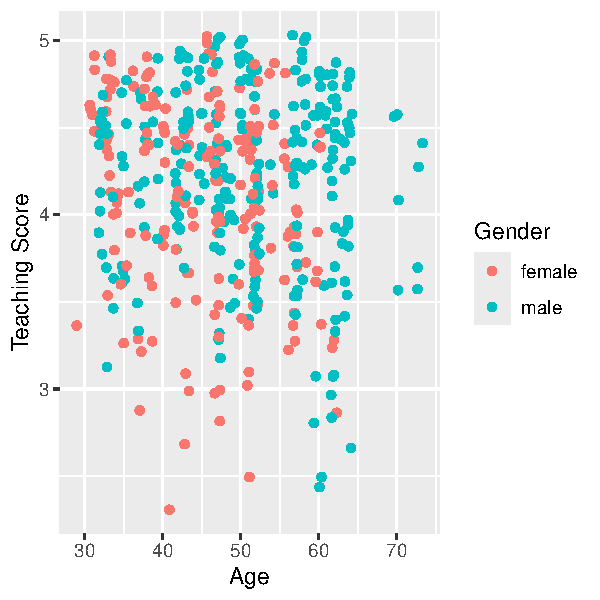
\includegraphics{notes_files/figure-pdf/unnamed-chunk-6-1.pdf}

}

\caption{Instructor evaluation scores by age and gender. The points have
been jittered.}

\end{figure}%

\begin{tcolorbox}[enhanced jigsaw, colback=white, toptitle=1mm, bottomrule=.15mm, colbacktitle=quarto-callout-note-color!10!white, breakable, title=\textcolor{quarto-callout-note-color}{\faInfo}\hspace{0.5em}{Note}, colframe=quarto-callout-note-color-frame, opacitybacktitle=0.6, toprule=.15mm, arc=.35mm, coltitle=black, leftrule=.75mm, bottomtitle=1mm, titlerule=0mm, opacityback=0, rightrule=.15mm, left=2mm]

The above code has jittered the points, however, this is not necessary
and \texttt{geom\_point} would suffice. To plot separate points by
gender we simply add the \texttt{color} argument to the \texttt{aes}
function and pass to it \texttt{gender}.

\end{tcolorbox}

From the scatterplot we can see that there are very few women over the
age of 60 in our data set and that the variability for women seems to be
slighlty larger than for men.

\subsection{Multiple regression: parallel slopes
model}\label{multiple-regression-parallel-slopes-model}

Here, we shall begin by fitting what is referred to as a parallel
regression lines model. This model implies that the slope of
relationship between teaching score (\texttt{score}) and age
(\texttt{age}) is the same for both males and females, with only the
intercept of the regression lines changing. Hence, our parallel
regression lines model is given as:

\begin{equation}\phantomsection\label{eq-parallel.lm}{
\begin{aligned}
y_{i} &= \alpha + \beta_1 x_{1i} + \beta_2 x_{2i} + \epsilon_i \nonumber \\&= \alpha + \beta_{\text{age}} \cdot \text{age} + \beta_{\text{male}} \cdot \mathbb{I}_{\text{male}}(x) + \epsilon_i, 
\end{aligned}
}\end{equation}

where

\begin{itemize}
\item
  \(\alpha\) is the intercept of the regression line for females;
\item
  \(\beta_{\text{age}}\) is the slope of the regression line for both
  males and females;
\item
  \(\beta_{\text{male}}\) is the additional term added to \(\alpha\) to
  get the intercept of the regression line for males; and
\item
  \(\mathbb{I}_{\text{male}}(x)\) is an indicator function such that

  \[\mathbb{I}_{\text{male}}(x)=\left\{
              \begin{array}{ll}
                1 ~~~ \text{if gender} ~ x ~ \text{is male},\\
                0 ~~~ \text{Otherwise}.\\
              \end{array}
            \right.\]
\end{itemize}

We can fit the parallel regression lines model as follows:

\begin{Shaded}
\begin{Highlighting}[]
\NormalTok{par.model }\OtherTok{\textless{}{-}} \FunctionTok{lm}\NormalTok{(score }\SpecialCharTok{\textasciitilde{}}\NormalTok{ age }\SpecialCharTok{+}\NormalTok{ gender, }\AttributeTok{data =}\NormalTok{ eval.score)}
\FunctionTok{tab\_model}\NormalTok{(par.model,}\AttributeTok{show.ci =}\NormalTok{ F)}
\end{Highlighting}
\end{Shaded}

\begin{longtable}[]{@{}ccc@{}}
\toprule\noalign{}
\endhead
\bottomrule\noalign{}
\endlastfoot
~ & \multicolumn{2}{c@{}}{%
score} \\
Predictors & Estimates & p \\
(Intercept) & 4.48 & \textbf{\textless0.001} \\
age & -0.01 & \textbf{0.001} \\
gender {[}male{]} & 0.19 & \textbf{\textless0.001} \\
Observations & \multicolumn{2}{l@{}}{%
463} \\
R\textsuperscript{2} / R\textsuperscript{2} adjusted &
\multicolumn{2}{l@{}}{%
0.039 / 0.035} \\
\end{longtable}

Hence, the regression line for females is given by:

\[\widehat{\text{score}} = 4.48 - 0.01 \cdot \text{age},\]

while the regression line for males is given by:

\[\widehat{\text{score}} = 4.48 - 0.01 \cdot \text{age} + 0.191 = 4.671 - 0.009 \cdot \text{age}.\]

Now, let's superimpose our parallel regression lines onto the
scatterplot of teaching score against age. To do so we will use the
\texttt{plot\_model} function from the \texttt{sjPlot} library as
follows:

\begin{Shaded}
\begin{Highlighting}[]
\FunctionTok{plot\_model}\NormalTok{(}\AttributeTok{model =}\NormalTok{ par.model,                 }\CommentTok{\# The fitted model}
           \AttributeTok{type=}\StringTok{"pred"}\NormalTok{,               }\CommentTok{\# type of plot}
           \AttributeTok{terms =} \FunctionTok{c}\NormalTok{(}\StringTok{"age"}\NormalTok{,}\StringTok{"gender"}\NormalTok{), }\CommentTok{\# terms to include in the plot}
           \AttributeTok{grid=}\NormalTok{T,                    }\CommentTok{\# split into a grid}
           \AttributeTok{show.data =}\NormalTok{ T,             }\CommentTok{\# show observations}
           \AttributeTok{jitter=}\NormalTok{T,                  }\CommentTok{\# jitter the points}
           \AttributeTok{ci.lvl =} \ConstantTok{NA}\NormalTok{,               }\CommentTok{\# show/hide confidence intervals}
           \AttributeTok{title=}\StringTok{"Parallel Regression Model fitted lines"}\NormalTok{) }\CommentTok{\# Plot title}
\end{Highlighting}
\end{Shaded}

\begin{figure}[H]

{\centering 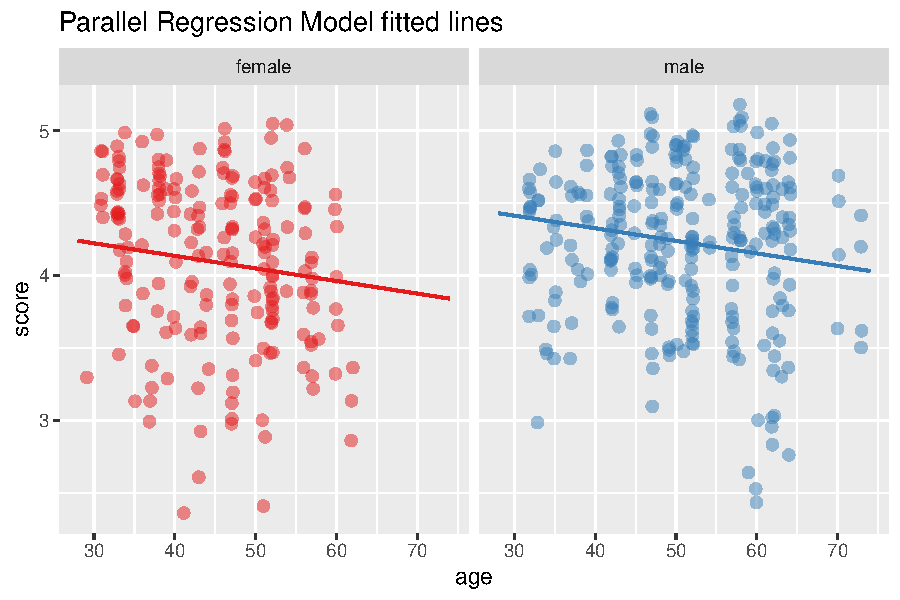
\includegraphics{notes_files/figure-pdf/unnamed-chunk-7-1.pdf}

}

\caption{Instructor evaluation scores by age and gender with parallel
regression lines superimposed.}

\end{figure}%

Here is a short description of the \texttt{plot\_model} function
arguments we have used:

\begin{itemize}
\item
  \texttt{model} is the fitted \texttt{lm}-class model.
\item
  \texttt{type\ =\ "pred"} plot the predicted values for specific model
  terms.
\item
  \texttt{terms\ =\ c("age","gender")} the terms to be plotted
\item
  \texttt{grid=T} logical argument to plot the different fitted lines
  for each group (i.e., gender) on different panels
\item
  \texttt{show.data=T} and \texttt{jitter=T} logical arguments to show
  our observations and jitter the data points.
\item
  \texttt{ci.lvl} set to \texttt{NA} to hide the confidence bands (we
  will talk more about this later)
\item
  \texttt{title} title for the plot.
\end{itemize}

From the parallel regression lines model both males and females have the
same slope, that is, the associated effect of age on teaching score is
the same for both men and women. Hence, for every one year increase in
age, there is an associated decrease in teaching score of 0.009.
However, male instructors have a higher intercept term, that is, there
is a vertical bump in the regression line for males in teaching scores.
This is linked to the average difference in teaching scores that males
obtain relative to females.

\subsection{Multiple regression: interaction
model}\label{multiple-regression-interaction-model}

There is an \emph{interaction effect} if the associated effect of one
variable depends on the value of another variable. For example, the
effect of age here will depend on whether the instructor is male or
female, that is, the effect of age on teaching scores will differ by
gender. The interaction model can be written as:

\begin{equation}\phantomsection\label{eq-inter.lm}{
\begin{aligned}
y_{i} &= \alpha + \beta_1  x_{1i} + \beta_2  x_{2i} + \beta_3  x_{1i}  x_{2i} + \epsilon_i \nonumber \\&= \alpha + \beta_{\text{age}} \cdot \text{age} + \beta_{\text{male}} \cdot \mathbb{I}_{\text{male}}(x) + \beta_{\text{age, male}} \cdot \text{age} \cdot \mathbb{I}_{\text{male}}(x) + \epsilon_i, 
\end{aligned}
}\end{equation}

where
\(\beta_{\text{age, male}} \cdot \text{age} \cdot \mathbb{I}_{\text{male}}(x)\)
corresponds to the interaction term.

In order to fit an interaction term within our regression model we
replace the \texttt{+} sign with the \texttt{*} sign as follows:

\begin{Shaded}
\begin{Highlighting}[]
\NormalTok{int.model }\OtherTok{\textless{}{-}}\FunctionTok{lm}\NormalTok{(score }\SpecialCharTok{\textasciitilde{}}\NormalTok{ age }\SpecialCharTok{*}\NormalTok{ gender, }\AttributeTok{data =}\NormalTok{ eval.score)}
\FunctionTok{tab\_model}\NormalTok{(int.model,}\AttributeTok{show.ci =}\NormalTok{ F)}
\end{Highlighting}
\end{Shaded}

\begin{longtable}[]{@{}ccc@{}}
\toprule\noalign{}
\endhead
\bottomrule\noalign{}
\endlastfoot
~ & \multicolumn{2}{c@{}}{%
score} \\
Predictors & Estimates & p \\
(Intercept) & 4.88 & \textbf{\textless0.001} \\
age & -0.02 & \textbf{\textless0.001} \\
gender {[}male{]} & -0.45 & 0.094 \\
age × gender {[}male{]} & 0.01 & \textbf{0.015} \\
Observations & \multicolumn{2}{l@{}}{%
463} \\
R\textsuperscript{2} / R\textsuperscript{2} adjusted &
\multicolumn{2}{l@{}}{%
0.051 / 0.045} \\
\end{longtable}

Hence, the regression line for females is given by:

\[\widehat{\text{score}} = 4.88 - 0.018 \cdot \text{age},\] while the
regression line for males is given by:

\[\widehat{\text{score}} = 4.88 - 0.018 \cdot \text{age} - 0.446 + 0.014 \cdot \text{age} = 4.434 - 0.004 \cdot \text{age}.\]

\begin{tcolorbox}[enhanced jigsaw, colback=white, toptitle=1mm, bottomrule=.15mm, colbacktitle=quarto-callout-tip-color!10!white, breakable, title={Question}, colframe=quarto-callout-tip-color-frame, opacitybacktitle=0.6, toprule=.15mm, arc=.35mm, coltitle=black, leftrule=.75mm, bottomtitle=1mm, titlerule=0mm, opacityback=0, rightrule=.15mm, left=2mm]

How do they compare with the teaching score values from the parallel
regression lines model?

Answer

Here, we can see that, although the intercept for male instructors may
be lower, the associated average decrease in teaching score with age
(0.004) is not as severe as it is for female instructors (0.018).

\end{tcolorbox}

We can plot the fitted model as we did before with the
\texttt{plot\_model} function. Lets try it now without the panel option
(i.e., set \texttt{grid\ =\ F}) and selecting our color scheme:

\begin{Shaded}
\begin{Highlighting}[]
\FunctionTok{plot\_model}\NormalTok{(}\AttributeTok{model =}\NormalTok{ int.model,         }\CommentTok{\# The fitted intertaction model}
           \AttributeTok{type=}  \StringTok{"pred"}\NormalTok{,              }\CommentTok{\# type of plot}
           \AttributeTok{terms =} \FunctionTok{c}\NormalTok{(}\StringTok{"age"}\NormalTok{,}\StringTok{"gender"}\NormalTok{), }\CommentTok{\# terms to include in the plot}
           \AttributeTok{grid=}\NormalTok{F,                    }\CommentTok{\# split into a grid}
           \AttributeTok{show.data =}\NormalTok{ T,             }\CommentTok{\# show observations}
           \AttributeTok{jitter=}\NormalTok{T,                  }\CommentTok{\# jitter the points}
           \AttributeTok{ci.lvl =} \ConstantTok{NA}\NormalTok{,               }\CommentTok{\# show/hide confidence intervals}
           \AttributeTok{title =}\StringTok{"Gender{-}age interaction model fitted lines"}\NormalTok{, }\CommentTok{\# Plot title}
           \AttributeTok{colors =} \FunctionTok{c}\NormalTok{(}\StringTok{"purple"}\NormalTok{, }\StringTok{"orange"}\NormalTok{)) }\CommentTok{\# color scheme}
\end{Highlighting}
\end{Shaded}

\begin{figure}[H]

{\centering 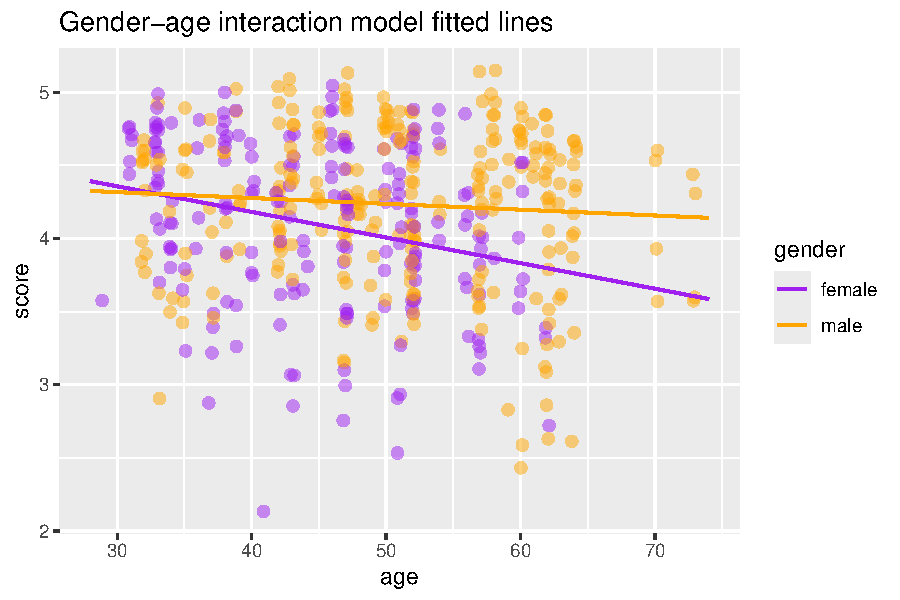
\includegraphics{notes_files/figure-pdf/unnamed-chunk-9-1.pdf}

}

\caption{Instructor evaluation scores by age and gender with
gender-varying regression lines superimposed.}

\end{figure}%

\subsection{Assessing model fit}\label{assessing-model-fit}

Now we have to assess the fit of the model by looking at plots of the
residuals. We shall do this for the interaction model. First, we need to
obtain the fitted values and residuals from the interaction model as
follows:

\begin{Shaded}
\begin{Highlighting}[]
\NormalTok{int.model\_output }\OtherTok{\textless{}{-}}\NormalTok{  eval.score }\SpecialCharTok{\%\textgreater{}\%} 
  \FunctionTok{mutate}\NormalTok{(}\AttributeTok{score\_hat  =}\NormalTok{ int.model}\SpecialCharTok{$}\NormalTok{fitted.values,}
         \AttributeTok{residual =}\NormalTok{ int.model}\SpecialCharTok{$}\NormalTok{residuals)}
\end{Highlighting}
\end{Shaded}

Let's start by looking at a scatterplot of the residuals against the
explanatory variable by gender:

\begin{Shaded}
\begin{Highlighting}[]
\FunctionTok{ggplot}\NormalTok{(int.model\_output, }\FunctionTok{aes}\NormalTok{(}\AttributeTok{x =}\NormalTok{ age, }\AttributeTok{y =}\NormalTok{ residual)) }\SpecialCharTok{+}
  \FunctionTok{geom\_point}\NormalTok{() }\SpecialCharTok{+}
  \FunctionTok{labs}\NormalTok{(}\AttributeTok{x =} \StringTok{"age"}\NormalTok{, }\AttributeTok{y =} \StringTok{"Residual"}\NormalTok{) }\SpecialCharTok{+}
  \FunctionTok{geom\_hline}\NormalTok{(}\AttributeTok{yintercept =} \DecValTok{0}\NormalTok{, }\AttributeTok{col =} \StringTok{"blue"}\NormalTok{, }\AttributeTok{linewidth =} \DecValTok{1}\NormalTok{) }\SpecialCharTok{+}
  \FunctionTok{facet\_wrap}\NormalTok{(}\SpecialCharTok{\textasciitilde{}}\NormalTok{ gender)}
\end{Highlighting}
\end{Shaded}

\begin{figure}[H]

{\centering 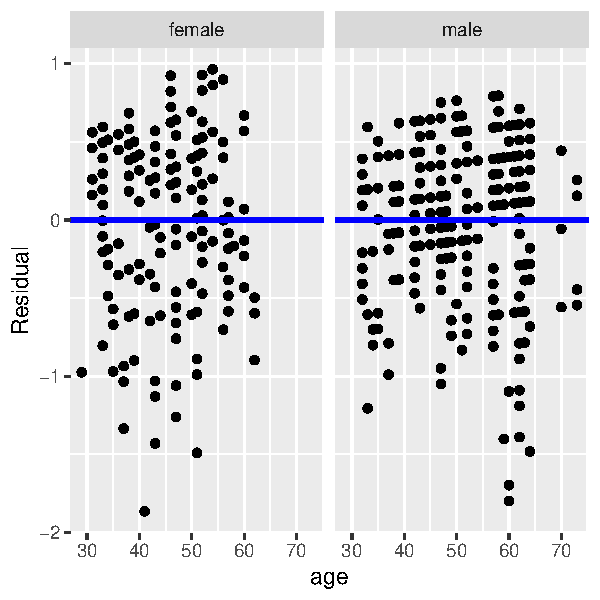
\includegraphics{notes_files/figure-pdf/unnamed-chunk-11-1.pdf}

}

\caption{Residuals vs the explanatory variable age by gender.}

\end{figure}%

Now, we can plot the residuals against the fitted values using either
the \texttt{check\_model} function from the \texttt{performance} package
or the \texttt{plot\_model()} from \texttt{sjPlot} by setting
\texttt{type="diag"}:

\section{\texorpdfstring{Using
\texttt{check\_model}}{Using check\_model}}

\begin{Shaded}
\begin{Highlighting}[]
\FunctionTok{check\_model}\NormalTok{(int.model,}\AttributeTok{check =} \FunctionTok{c}\NormalTok{(}\StringTok{"linearity"}\NormalTok{,}\StringTok{"homogeneity"}\NormalTok{))}
\end{Highlighting}
\end{Shaded}

\begin{center}
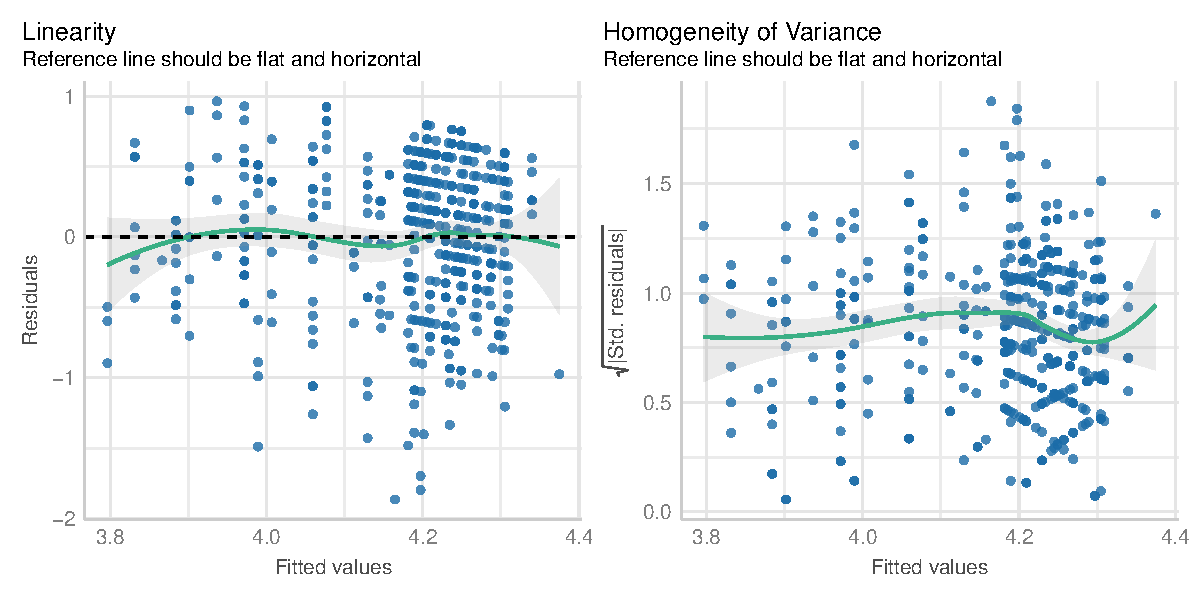
\includegraphics{notes_files/figure-pdf/unnamed-chunk-12-1.pdf}
\end{center}

\section{\texorpdfstring{Using \texttt{plot\_model}}{Using plot\_model}}

\begin{Shaded}
\begin{Highlighting}[]
\NormalTok{int.model\_diag }\OtherTok{\textless{}{-}} \FunctionTok{plot\_model}\NormalTok{(int.model,}\AttributeTok{type =} \StringTok{"diag"}\NormalTok{)}
\NormalTok{int.model\_diag[[}\DecValTok{4}\NormalTok{]]}
\end{Highlighting}
\end{Shaded}

\begin{center}
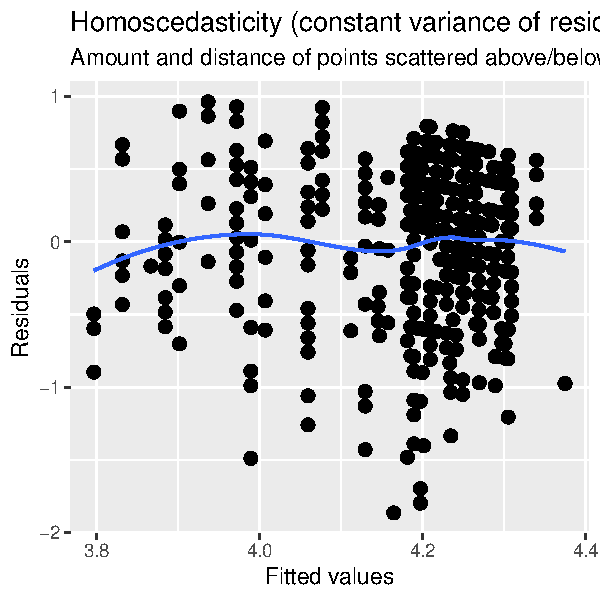
\includegraphics{notes_files/figure-pdf/unnamed-chunk-13-1.pdf}
\end{center}

\newpage

Finally, let's plot histograms of the residuals and QQ-plots to assess
whether they are normally distributed with mean zero:

\section{\texorpdfstring{Using
\texttt{check\_model}}{Using check\_model}}

\begin{Shaded}
\begin{Highlighting}[]
\FunctionTok{check\_model}\NormalTok{(int.model,}\AttributeTok{check =} \FunctionTok{c}\NormalTok{(}\StringTok{"qq"}\NormalTok{,}\StringTok{"normality"}\NormalTok{))}
\end{Highlighting}
\end{Shaded}

\begin{center}
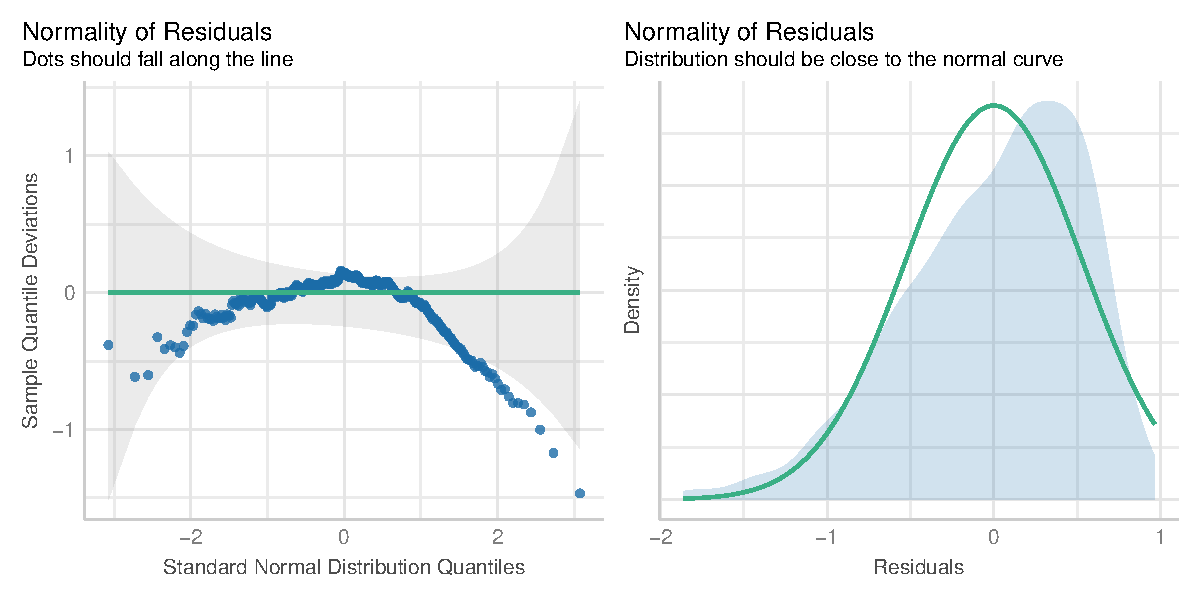
\includegraphics{notes_files/figure-pdf/unnamed-chunk-14-1.pdf}
\end{center}

\section{\texorpdfstring{Using \texttt{plot\_model}}{Using plot\_model}}

\begin{Shaded}
\begin{Highlighting}[]
\FunctionTok{library}\NormalTok{(gridExtra) }\CommentTok{\# to arrange the plots side{-}by{-}side}
\NormalTok{int.model\_diag }\OtherTok{\textless{}{-}} \FunctionTok{plot\_model}\NormalTok{(int.model,}\AttributeTok{type =} \StringTok{"diag"}\NormalTok{)}

\NormalTok{gridExtra}\SpecialCharTok{::}\FunctionTok{grid.arrange}\NormalTok{(int.model\_diag[[}\DecValTok{2}\NormalTok{]], }\CommentTok{\# qqplot}
\NormalTok{                        int.model\_diag[[}\DecValTok{3}\NormalTok{]], }\CommentTok{\# histogram}
                        \AttributeTok{ncol=}\DecValTok{2}\NormalTok{) }\CommentTok{\# plot them side by side}
\end{Highlighting}
\end{Shaded}

\begin{center}
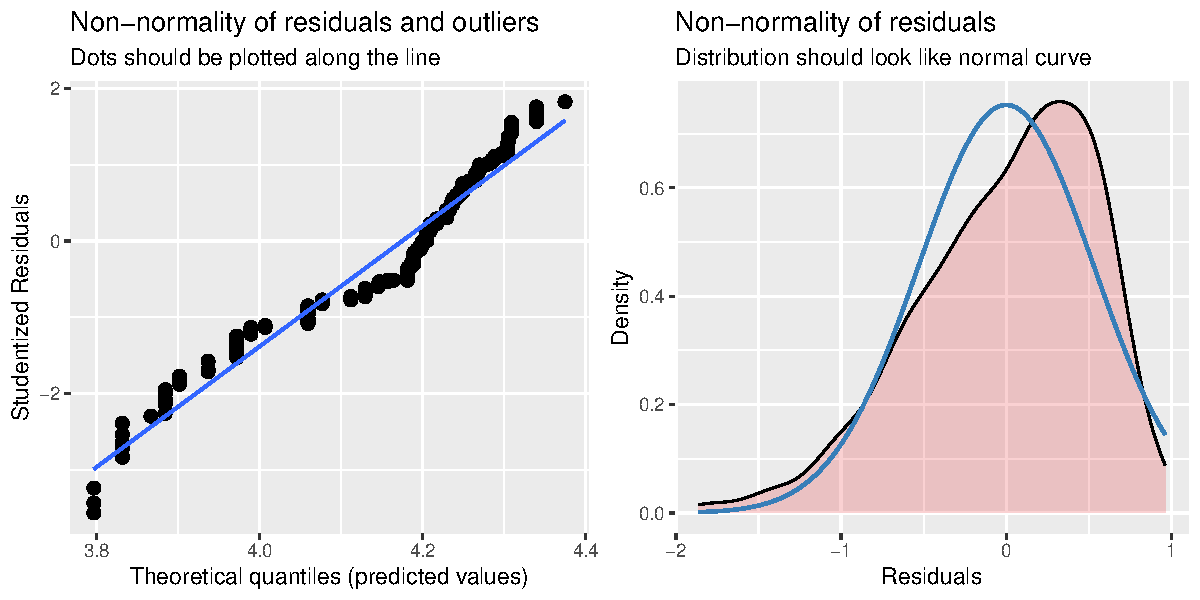
\includegraphics{notes_files/figure-pdf/unnamed-chunk-15-1.pdf}
\end{center}

\begin{tcolorbox}[enhanced jigsaw, colback=white, toptitle=1mm, bottomrule=.15mm, colbacktitle=quarto-callout-warning-color!10!white, breakable, title={Task 2}, colframe=quarto-callout-warning-color-frame, opacitybacktitle=0.6, toprule=.15mm, arc=.35mm, coltitle=black, leftrule=.75mm, bottomtitle=1mm, titlerule=0mm, opacityback=0, rightrule=.15mm, left=2mm]

Using \texttt{ggplot} to produce manually:

\begin{enumerate}
\def\labelenumi{\arabic{enumi}.}
\tightlist
\item
  a scatter plot of the residuals vs.~fitted values
\item
  histogram of the residuals to assess normality
\end{enumerate}

Take a hint

The \texttt{int.model\_output} data we produced above contains all the
information you need. Recall that a scatterplots and histograms can be
produced with \texttt{geom\_point} and \texttt{geom\_histogram} layers
respectively.

Click here to see the solution

\begin{Shaded}
\begin{Highlighting}[]
\NormalTok{p1 }\OtherTok{\textless{}{-}} \FunctionTok{ggplot}\NormalTok{(int.model\_output,}
             \FunctionTok{aes}\NormalTok{(}\AttributeTok{y=}\NormalTok{residual,}\AttributeTok{x=}\NormalTok{score\_hat))}\SpecialCharTok{+}
  \FunctionTok{geom\_point}\NormalTok{()}\SpecialCharTok{+}
  \FunctionTok{labs}\NormalTok{(}\AttributeTok{y=}\StringTok{"Residuals"}\NormalTok{,}\AttributeTok{x=}\StringTok{"Fitted values"}\NormalTok{)}
\NormalTok{p2 }\OtherTok{\textless{}{-}} \FunctionTok{ggplot}\NormalTok{(int.model\_output,}
             \FunctionTok{aes}\NormalTok{(}\AttributeTok{x=}\NormalTok{residual))}\SpecialCharTok{+}
  \FunctionTok{geom\_histogram}\NormalTok{()}
\NormalTok{gridExtra}\SpecialCharTok{::}\FunctionTok{grid.arrange}\NormalTok{(p1, }\CommentTok{\# resid. vs. fitted}
\NormalTok{                        p2, }\CommentTok{\# histogram}
                        \AttributeTok{ncol=}\DecValTok{2}\NormalTok{)}
\end{Highlighting}
\end{Shaded}

\begin{center}
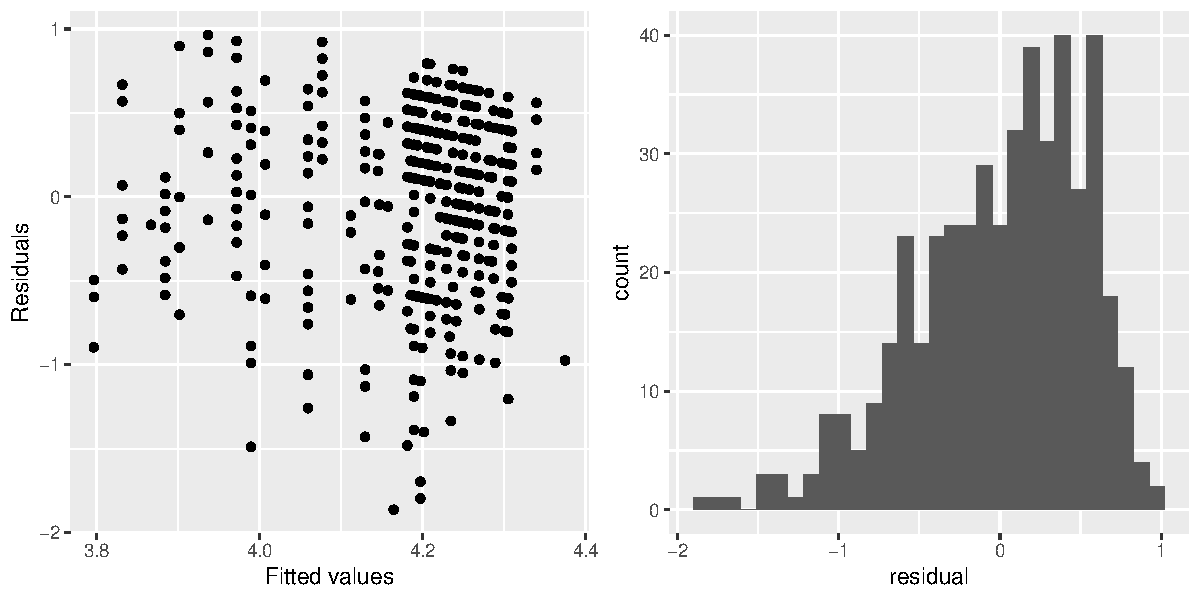
\includegraphics{notes_files/figure-pdf/unnamed-chunk-16-1.pdf}
\end{center}

\end{tcolorbox}

\section{Sample statistics}\label{sample-statistics}

This week, and in previous weeks, we have seen many examples of
calculating \emph{sample statistics} such as means, percentiles,
standard deviations and regression coefficients. These \emph{sample
statistics} are used as \emph{point estimates} of \emph{population
parameters} which describe the \emph{population} from which the
\emph{sample} of data was taken. That last sentence assumes you're
familiar with concepts and terminology about sampling (e.g.~from the
\emph{Statistical Inference} course) so here is a summary of some key
terms:

\begin{enumerate}
\def\labelenumi{\arabic{enumi}.}
\item
  \textbf{Population}: The population is a set of \(N\) observations of
  interest.
\item
  \textbf{Population parameter}: A population parameter is a numerical
  summary value about the population. In most settings, this is a value
  that's unknown and you wish you knew it.
\item
  \textbf{Census}: An exhaustive enumeration/counting of all
  observations in the population in order to compute the population
  parameter's numerical value \emph{exactly}.

  \begin{itemize}
  \tightlist
  \item
    When \(N\) is small, a census is feasible. However, when \(N\) is
    large, a census can get very expensive, either in terms of time,
    energy, or money.
  \end{itemize}
\item
  \textbf{Sampling}: Collecting a sample of size \(n\) of observations
  from the population. Typically the sample size \(n\) is much smaller
  than the population size \(N\), thereby making sampling a much cheaper
  procedure than a census.

  \begin{itemize}
  \tightlist
  \item
    It is important to remember that the lowercase \(n\) corresponds to
    the sample size and uppercase \(N\) corresponds to the population
    size, thus \(n \leq N\).
  \end{itemize}
\item
  \textbf{Point estimates/sample statistics}: A summary statistic based
  on the sample of size \(n\) that \emph{estimates} the unknown
  population parameter.
\item
  \textbf{Representative sampling}: A sample is said be a
  \emph{representative sample} if it ``looks like the population''. In
  other words, the sample's characteristics are a good representation of
  the population's characteristics.
\item
  \textbf{Generalisability}: We say a sample is \emph{generalisable} if
  any results based on the sample can generalise to the population.
\item
  \textbf{Bias}: In a statistical sense, we say \emph{bias} occurs if
  certain observations in a population have a higher chance of being
  sampled than others. We say a sampling procedure is \emph{unbiased} if
  every observation in a population had an equal chance of being
  sampled.
\item
  \textbf{Random sampling}: We say a sampling procedure is \emph{random}
  if we sample randomly from the population in an unbiased fashion.
\end{enumerate}

\subsection{Inference using sample
statistics}\label{inference-using-sample-statistics}

The table below lists a variety of contexts where sample statistics can
be used to estimate population parameters. In all 6 cases, the point
estimate/sample statistic \emph{estimates} the unknown population
parameter. It does so by computing summary statistics based on a sample
of size \(n\). We'll cover Scenarios 5 and 6, namely construct CIs for
the parameters in simple and multiple linear regression models. We will
consider CIs based on theoretical results when standard assumptions
hold, although sampling procedures such as bootstrap also exist. We will
also consider how to use CIs for variable selection and finish by
considering a model selection strategy based on objective measures for
model comparisons.

Table 1: Scenarios of sample statistics for inference.

\begin{longtable}[]{@{}
  >{\raggedright\arraybackslash}p{(\columnwidth - 8\tabcolsep) * \real{0.0909}}
  >{\raggedright\arraybackslash}p{(\columnwidth - 8\tabcolsep) * \real{0.2091}}
  >{\raggedright\arraybackslash}p{(\columnwidth - 8\tabcolsep) * \real{0.1909}}
  >{\raggedright\arraybackslash}p{(\columnwidth - 8\tabcolsep) * \real{0.2091}}
  >{\raggedright\arraybackslash}p{(\columnwidth - 8\tabcolsep) * \real{0.3000}}@{}}
\toprule\noalign{}
\begin{minipage}[b]{\linewidth}\raggedright
Scenario
\end{minipage} & \begin{minipage}[b]{\linewidth}\raggedright
Population Parameter
\end{minipage} & \begin{minipage}[b]{\linewidth}\raggedright
Population Notation
\end{minipage} & \begin{minipage}[b]{\linewidth}\raggedright
Sample Statistic
\end{minipage} & \begin{minipage}[b]{\linewidth}\raggedright
Sample Notation
\end{minipage} \\
\midrule\noalign{}
\endhead
\bottomrule\noalign{}
\endlastfoot
1 & Population proportion & \(p\) & Sample proportion &
\(\widehat{p}\) \\
2 & Population mean & \(\mu\) & Sample mean & \(\bar{x}\) \\
3 & Diff.in pop. props & \(p_1 - p_2\) & Diff. in sample props &
\(\widehat{p}_1 - \widehat{p}_2\) \\
4 & Diff. in pop. means & \(\mu_1 - \mu_2\) & Diff. in sample means &
\(\bar{x}_1 - \bar{x}_2\) \\
5 & Pop. intercept & \(\beta_0\) & Sample intercept &
\(\widehat{\beta}_0\) or \(b_0\) \\
6 & Pop. slope & \(\beta_1\) & Sample slope & \(\widehat{\beta}_1\) or
\(b_1\) \\
\end{longtable}

In reality, we don't have access to the population parameter values (if
we did, why would we need to estimate them?) we only have a single
sample of data from a larger population. We'd like to be able to make
some reasonable guesses about population parameters using that single
sample to create a range of plausible values for a population parameter.
This range of plausible values is known as a \textbf{confidence
interval}. The confidence intervals we will see this week are calculated
using the theoretical results based on the standard assumptions that you
will have seen in \emph{Regression Modelling}.

\section{Constructing confidence
intervals}\label{constructing-confidence-intervals}

A \textbf{confidence interval} gives a range of plausible values for a
population parameter. It depends on a specified \emph{confidence level}
with higher confidence levels corresponding to wider confidence
intervals and lower confidence levels corresponding to narrower
confidence intervals. Common confidence levels include 90\%, 95\%, and
99\%.

\textbf{Confidence intervals} are simple to define and play an important
role in the sciences and any field that uses data. You can think of a
confidence interval as playing the role of a net when fishing. Instead
of just trying to catch a fish with a single spear (estimating an
unknown parameter by using a single point estimate/sample statistic), we
can use a net to try to provide a range of possible locations for the
fish (use a range of possible values based around our sample statistic
to make a plausible guess as to the location of the parameter).

\subsection{Confidence Intervals for Regression
Parameters}\label{confidence-intervals-for-regression-parameters}

To illustrate this, let's have another look at teaching evaluations data
\texttt{evals} with the SLR model with \texttt{age} as the the single
explanatory variable and the instructors' evaluation \texttt{score}s as
the response variable. This data and the fitted model are shown here.

\begin{Shaded}
\begin{Highlighting}[]
\NormalTok{slr.model }\OtherTok{\textless{}{-}} \FunctionTok{lm}\NormalTok{(score }\SpecialCharTok{\textasciitilde{}}\NormalTok{ age, }\AttributeTok{data =}\NormalTok{ evals)}
\end{Highlighting}
\end{Shaded}

\begin{verbatim}
 (Intercept)          age 
 4.461932354 -0.005938225 
\end{verbatim}

\begin{figure}[H]

{\centering 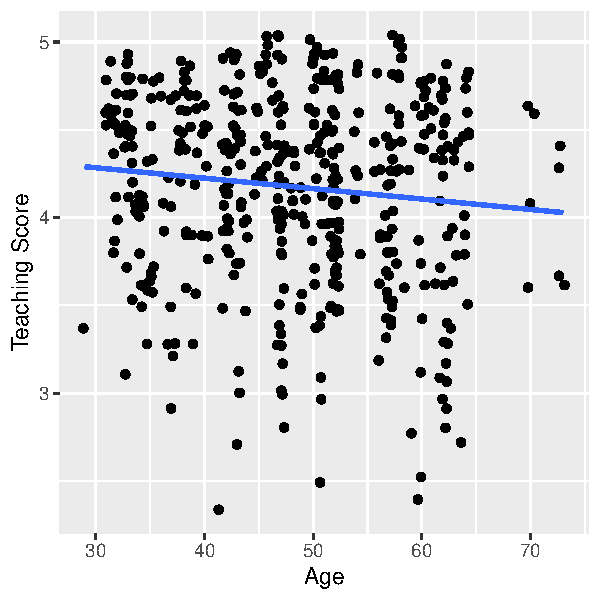
\includegraphics{notes_files/figure-pdf/unnamed-chunk-18-1.pdf}

}

\caption{SLR model applied to the teaching evaluation Data.}

\end{figure}%

The point estimate of the slope parameter here is \(\widehat{\beta}=\)
-0.006. But what about the uncertainty of our estimation? Well we can
construct confidence interval for this.

\textbf{Simple linear regression (SLR)}

\begin{tcolorbox}[enhanced jigsaw, colback=white, toptitle=1mm, bottomrule=.15mm, colbacktitle=quarto-callout-note-color!10!white, breakable, title=\textcolor{quarto-callout-note-color}{\faInfo}\hspace{0.5em}{Re-cap on SLR}, colframe=quarto-callout-note-color-frame, opacitybacktitle=0.6, toprule=.15mm, arc=.35mm, coltitle=black, leftrule=.75mm, bottomtitle=1mm, titlerule=0mm, opacityback=0, rightrule=.15mm, left=2mm]

Recall that for a simple linear regression model we have:

\begin{itemize}
\item
  \(\text{Var}(\hat{\beta}_0) = \sigma^2 \left[\frac{1}{n} + \frac{\bar{x}^2}{S_{xx}}\right]\)
  and
  \(se(\hat{\beta_0}) = \sqrt{\hat{\sigma^2} \left[\frac{1}{n} + \frac{\bar{x}^2}{S_{xx}}\right]}\)
\item
  \(\text{Var}(\hat{\beta}_1) = \frac{\sigma^2}{S_{xx}}\) and
  \(se(\hat{\beta_1}) = \frac{\hat{\sigma^2}}{S_{xx}}\)
\end{itemize}

Where \(S_{xx} = \sum_{i=1}^n (x_i-\bar{x})^2\) and
\(\hat{\sigma^2} = \frac{\sum_i y_i-\hat{y}}{n-2}\). Then, we get the
following pivotal quantities:

\[
\dfrac{\hat{\beta_j} - \beta_j}{se(\hat{\beta_j})} \sim t_{n-2}
\]for \(j \in \{0,1\}\).

\end{tcolorbox}

A \(100(1-\alpha)\)\% confidence interval for the intercept and slope is
given by:

\begin{itemize}
\item
  \(\hat{\beta_0} \pm t_{\alpha/2,n-2} \times se(\hat{\beta_0})\)
\item
  \(\hat{\beta_1} \pm t_{\alpha/2,n-2} \times se(\hat{\beta_1})\)
\end{itemize}

where \(t_{\alpha/2,n-2}\) is the critical t-value for a 95\% confidence
interval (note that sometimes a Gaussian approximation is used such that
\(\hat{\beta_j} \pm 1.96 \times se(\hat{\beta_j})\) - this assumes
\(\sigma^2\) is known).

\begin{quote}
A confidence interval gives a range of plausible values for a population
parameter.
\end{quote}

We can therefore use the confidence interval for \(\beta_1\) to state a
range of plausible values and, just as usefully, what values are
\textbf{not} plausible. The most common value to compare the confidence
interval of \(\beta_1\) with is 0 (zero), since \(\beta_1 = 0\) says
there is \emph{no} (linear) relationship between the response variable
(\(y\)) and the explanatory variable (\(x\)). Therefore, if 0 lies
within the confidence interval for \(\beta_1\) then there is
insufficient evidence of a linear relationship between \(y\) and \(x\).
However, if 0 \textbf{does not} lie within the confidence interval, then
we conclude that \(\beta_1\) is significantly different from zero and
therefore that there is evidence of a linear relationship between \(y\)
and \(x\).

Let's use the confidence interval based on theoretical results for the
slope parameter in the SLR model applied to the teacher evaluation
scores with \texttt{age} as the the single explanatory variable and the
instructors' evaluation \texttt{score}s as the outcome variable.

The \texttt{tab\_model} function allow us to print the \((1-\alpha)\)\%
confidence intervals for our parameters using the argument
\texttt{show.ci\ =\ (1-alpha)}. Additionally, we can print the estimator
standard error by setting \texttt{show.se=T}):

\begin{Shaded}
\begin{Highlighting}[]
\FunctionTok{tab\_model}\NormalTok{(slr.model,}\AttributeTok{show.se =}\NormalTok{ T,}\AttributeTok{show.ci =} \FloatTok{0.95}\NormalTok{)}
\end{Highlighting}
\end{Shaded}

\begin{longtable}[]{@{}ccccc@{}}
\toprule\noalign{}
\endhead
\bottomrule\noalign{}
\endlastfoot
~ & \multicolumn{4}{c@{}}{%
score} \\
Predictors & Estimates & std. Error & CI & p \\
(Intercept) & 4.46 & 0.13 & 4.21~--~4.71 & \textbf{\textless0.001} \\
age & -0.01 & 0.00 & -0.01~--~-0.00 & \textbf{0.021} \\
Observations & \multicolumn{4}{l@{}}{%
463} \\
R\textsuperscript{2} / R\textsuperscript{2} adjusted &
\multicolumn{4}{l@{}}{%
0.011 / 0.009} \\
\end{longtable}

This will give you a nice looking html table. However, if you prefer
your output to be a \texttt{data.frame} object, you can use the
\texttt{tidy} function from the \texttt{broom} package instead (you can
print the CI using \texttt{conf.int=T}):

\begin{Shaded}
\begin{Highlighting}[]
\NormalTok{broom}\SpecialCharTok{::}\FunctionTok{tidy}\NormalTok{(slr.model,}\AttributeTok{conf.int=}\NormalTok{T,}\AttributeTok{conf.level =} \FloatTok{0.95}\NormalTok{)}
\end{Highlighting}
\end{Shaded}

\begin{verbatim}
# A tibble: 2 x 7
  term        estimate std.error statistic   p.value conf.low conf.high
  <chr>          <dbl>     <dbl>     <dbl>     <dbl>    <dbl>     <dbl>
1 (Intercept)  4.46      0.127       35.2  1.05e-132   4.21    4.71    
2 age         -0.00594   0.00257     -2.31 2.13e-  2  -0.0110 -0.000890
\end{verbatim}

Then we can plot our fitted SLR using the \texttt{plot\_model} function:

\begin{Shaded}
\begin{Highlighting}[]
\FunctionTok{plot\_model}\NormalTok{(}\AttributeTok{model =}\NormalTok{ slr.model,}
           \AttributeTok{terms =} \FunctionTok{c}\NormalTok{(}\StringTok{"age"}\NormalTok{),}
           \AttributeTok{type  =} \StringTok{"pred"}\NormalTok{,}
           \AttributeTok{title =} \StringTok{"Fitted Linear regression model"}\NormalTok{,}
           \AttributeTok{show.data =}\NormalTok{ T,}
           \AttributeTok{jitter =}\NormalTok{ T)}
\end{Highlighting}
\end{Shaded}

\begin{figure}[H]

{\centering 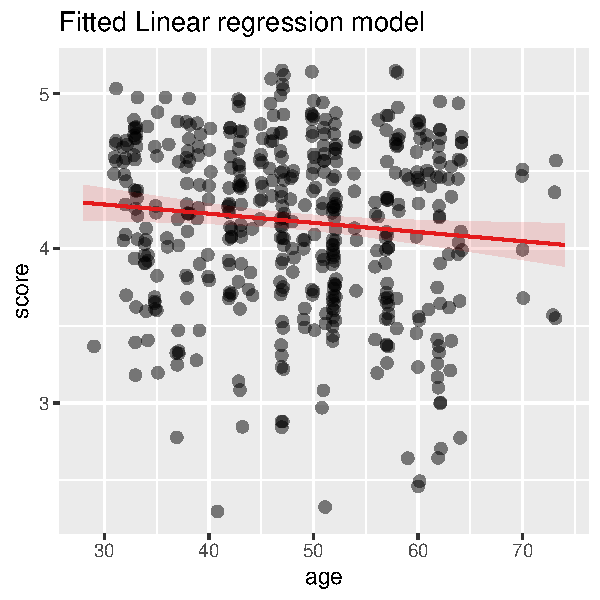
\includegraphics{notes_files/figure-pdf/unnamed-chunk-21-1.pdf}

}

\caption{SLR model applied to the teaching evaluation Data.}

\end{figure}%

\begin{tcolorbox}[enhanced jigsaw, colback=white, toptitle=1mm, bottomrule=.15mm, colbacktitle=quarto-callout-warning-color!10!white, breakable, title={Task 3}, colframe=quarto-callout-warning-color-frame, opacitybacktitle=0.6, toprule=.15mm, arc=.35mm, coltitle=black, leftrule=.75mm, bottomtitle=1mm, titlerule=0mm, opacityback=0, rightrule=.15mm, left=2mm]

Use \texttt{ggplot} to reproduce the plot above. You may achieve this by
adding a \texttt{geom\_smooth()} layer.

Hint

Chose \texttt{method\ ="lm"} as argument of the \texttt{geom\_smooth()}
layer. You may also chance the confidence level via the \texttt{level}
argument.

Click here to see the solution

\begin{Shaded}
\begin{Highlighting}[]
\FunctionTok{ggplot}\NormalTok{(evals, }\FunctionTok{aes}\NormalTok{(}\AttributeTok{x =}\NormalTok{ age, }\AttributeTok{y =}\NormalTok{ score)) }\SpecialCharTok{+}
  \FunctionTok{geom\_jitter}\NormalTok{() }\SpecialCharTok{+}
  \FunctionTok{labs}\NormalTok{(}\AttributeTok{x =} \StringTok{"Age"}\NormalTok{, }\AttributeTok{y =} \StringTok{"Teaching Score"}\NormalTok{) }\SpecialCharTok{+}
 \FunctionTok{geom\_smooth}\NormalTok{(}\AttributeTok{method =} \StringTok{"lm"}\NormalTok{,}\AttributeTok{level=}\NormalTok{.}\DecValTok{95}\NormalTok{)}
\end{Highlighting}
\end{Shaded}

\begin{verbatim}
`geom_smooth()` using formula = 'y ~ x'
\end{verbatim}

\begin{center}
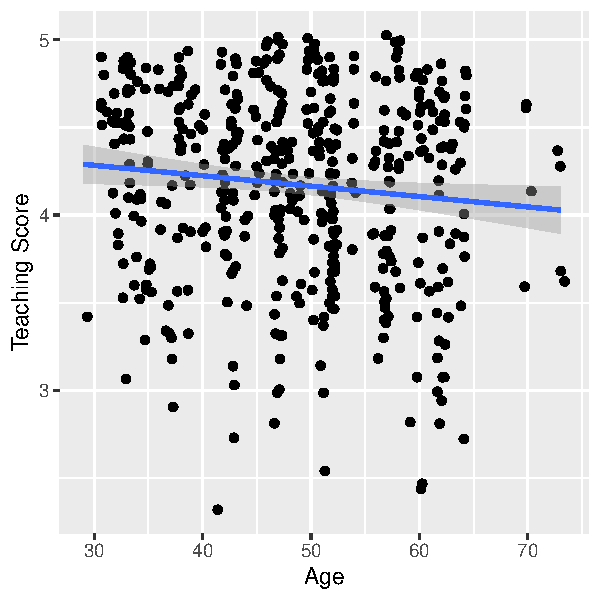
\includegraphics{notes_files/figure-pdf/unnamed-chunk-22-1.pdf}
\end{center}

\end{tcolorbox}

\textbf{Multiple Regression confidence intervals}

Let's continue with the teaching evaluations data by looking into the
multiple regression models we have fitted with one numerical and one
categorical explanatory variable . In these models:

\begin{itemize}
\tightlist
\item
  \(y\): response variable of instructor evaluation \texttt{score}
\item
  explanatory variables

  \begin{itemize}
  \tightlist
  \item
    \(x_1\): numerical explanatory variable of \texttt{age}
  \item
    \(x_2\): categorical explanatory variable of \texttt{gender}
  \end{itemize}
\end{itemize}

First, recall that we had two competing potential models to explain
professors' teaching evaluation scores:

\begin{enumerate}
\def\labelenumi{\arabic{enumi}.}
\tightlist
\item
  Model 1 ( Equation~\ref{eq-parallel.lm} ): Parallel lines model (no
  interaction term) - both male and female professors have the same
  slope describing the associated effect of age on teaching score
\item
  Model 2 ( Equation~\ref{eq-inter.lm} ): Interaction model - allowing
  for male and female professors to have different slopes describing the
  associated effect of age on teaching score
\end{enumerate}

Let's recall the output of these regression models:

\begin{Shaded}
\begin{Highlighting}[]
\FunctionTok{tab\_model}\NormalTok{(par.model,}
\NormalTok{          int.model,}
          \AttributeTok{collapse.ci =}\NormalTok{ T,}
          \AttributeTok{show.stat =}\NormalTok{ T,}
          \AttributeTok{show.se =}\NormalTok{ T,}
          \AttributeTok{dv.labels =} \FunctionTok{c}\NormalTok{(}\StringTok{"parallel lines model"}\NormalTok{,}\StringTok{"interaction model"}\NormalTok{) )}
\end{Highlighting}
\end{Shaded}

\begin{longtable}[]{@{}
  >{\centering\arraybackslash}p{(\columnwidth - 16\tabcolsep) * \real{0.1111}}
  >{\centering\arraybackslash}p{(\columnwidth - 16\tabcolsep) * \real{0.1111}}
  >{\centering\arraybackslash}p{(\columnwidth - 16\tabcolsep) * \real{0.1111}}
  >{\centering\arraybackslash}p{(\columnwidth - 16\tabcolsep) * \real{0.1111}}
  >{\centering\arraybackslash}p{(\columnwidth - 16\tabcolsep) * \real{0.1111}}
  >{\centering\arraybackslash}p{(\columnwidth - 16\tabcolsep) * \real{0.1111}}
  >{\centering\arraybackslash}p{(\columnwidth - 16\tabcolsep) * \real{0.1111}}
  >{\centering\arraybackslash}p{(\columnwidth - 16\tabcolsep) * \real{0.1111}}
  >{\centering\arraybackslash}p{(\columnwidth - 16\tabcolsep) * \real{0.1111}}@{}}
\toprule\noalign{}
\endhead
\bottomrule\noalign{}
\endlastfoot
~ &
\multicolumn{4}{>{\centering\arraybackslash}p{(\columnwidth - 16\tabcolsep) * \real{0.4444} + 6\tabcolsep}}{%
parallel lines model} &
\multicolumn{4}{>{\centering\arraybackslash}p{(\columnwidth - 16\tabcolsep) * \real{0.4444} + 6\tabcolsep}@{}}{%
interaction model} \\
Predictors & Estimates & std. Error & Statistic & p & Estimates & std.
Error & Statistic & p \\
(Intercept) & \begin{minipage}[t]{\linewidth}\raggedright
4.48\\
(4.24~--~4.73)\strut
\end{minipage} & 0.13 & 35.79 & \textbf{\textless0.001} &
\begin{minipage}[t]{\linewidth}\raggedright
4.88\\
(4.48~--~5.29)\strut
\end{minipage} & 0.21 & 23.80 & \textbf{\textless0.001} \\
age & \begin{minipage}[t]{\linewidth}\raggedright
-0.01\\
(-0.01~--~-0.00)\strut
\end{minipage} & 0.00 & -3.28 & \textbf{0.001} &
\begin{minipage}[t]{\linewidth}\raggedright
-0.02\\
(-0.03~--~-0.01)\strut
\end{minipage} & 0.00 & -3.92 & \textbf{\textless0.001} \\
gender {[}male{]} & \begin{minipage}[t]{\linewidth}\raggedright
0.19\\
(0.09~--~0.29)\strut
\end{minipage} & 0.05 & 3.63 & \textbf{\textless0.001} &
\begin{minipage}[t]{\linewidth}\raggedright
-0.45\\
(-0.97~--~0.08)\strut
\end{minipage} & 0.27 & -1.68 & 0.094 \\
age × gender {[}male{]} & & & & &
\begin{minipage}[t]{\linewidth}\raggedright
0.01\\
(0.00~--~0.02)\strut
\end{minipage} & 0.01 & 2.45 & \textbf{0.015} \\
Observations &
\multicolumn{4}{>{\raggedright\arraybackslash}p{(\columnwidth - 16\tabcolsep) * \real{0.4444} + 6\tabcolsep}}{%
463} &
\multicolumn{4}{>{\raggedright\arraybackslash}p{(\columnwidth - 16\tabcolsep) * \real{0.4444} + 6\tabcolsep}@{}}{%
463} \\
R\textsuperscript{2} / R\textsuperscript{2} adjusted &
\multicolumn{4}{>{\raggedright\arraybackslash}p{(\columnwidth - 16\tabcolsep) * \real{0.4444} + 6\tabcolsep}}{%
0.039 / 0.035} &
\multicolumn{4}{>{\raggedright\arraybackslash}p{(\columnwidth - 16\tabcolsep) * \real{0.4444} + 6\tabcolsep}@{}}{%
0.051 / 0.045} \\
\end{longtable}

Notice that, together with the estimated parameter values, the tables we
produced now include other information about each estimated parameter in
the model, namely:

\begin{itemize}
\tightlist
\item
  \textbf{std\_error}: the standard error of each parameter estimate
  (set \texttt{show.se\ =\ T});
\item
  \textbf{statistic}: the test statistic value used to test the null
  hypothesis that the population parameter is zero (set
  \texttt{show.stat\ =\ T});
\item
  \textbf{p\_value}: the \(p\) value associated with the test statistic
  under the null hypothesis; and
\item
  \textbf{lower\_ci} and \textbf{upper\_ci}: the lower and upper bounds
  of the 95\% confidence interval for the population parameter (the
  options \texttt{collapse.ci\ =T} can be used to parse the CI next to
  the parameter estimates)
\end{itemize}

These values are calculated using the theoretical results based on the
standard assumptions that you will have seen in \emph{Regression
Modelling}.

\section{Variable selection using confidence
intervals}\label{variable-selection-using-confidence-intervals}

When there is more than one explanatory variable in a model, the
parameter associated with each explanatory variable is interpreted as
the change in the mean response based on a 1-unit change in the
corresponding explanatory variable \textbf{keeping all other variables
held constant}. Therefore, care must be taken when interpreting the
confidence intervals of each parameter by acknowledging that each are
plausible values \textbf{conditional on all the other explanatory
variables in the model}.

Because of the interdependence between the parameter estimates and the
variables included in the model, choosing which variables to include in
the model is a rather complex task. We will introduce some of the ideas
in the simple case where we have 2 potential explanatory variables
(\(x_1\) and \(x_2\)) and use confidence intervals to decide which
variables will be useful in predicting the response variable.

One approach is to consider a hierarchy of models:

\[y_i = \alpha + \beta_1 x_{1i} + \beta_2 x_{2i}\]\\
\[y_i = \alpha + \beta_1 x_{1i} \qquad \qquad \qquad y_i = \alpha + \beta_2 x_{2i}\]\\
\[y_i = \alpha\]

Within this structure we might take a top-down approach:

\begin{enumerate}
\def\labelenumi{\arabic{enumi}.}
\tightlist
\item
  Fit the most general model,
  i.e.~\(y_i = \alpha + \beta_1 x_{1i} + \beta_2 x_{2i}\) since we
  believe this is likely to provide a good description of the data
\item
  Construct confidence intervals for \(\beta_1 ~\textrm{and} ~\beta_2\)

  \begin{enumerate}
  \def\labelenumii{(\alph{enumii})}
  \tightlist
  \item
    If both intervals exclude 0 then retain the model with both \(x_1\)
    and \(x_2\).
  \item
    If the interval for \(\beta_1\) contains 0 but that for \(\beta_2\)
    does not, fit the model with \(x_2\) alone.
  \item
    If the interval for \(\beta_2\) contains 0 but that for \(\beta_1\)
    does not, fit the model with \(x_1\) alone.
  \item
    If both intervals include 0 it may still be that a model with one
    variable is useful. In this case the two models with the single
    variables should be fitted and intervals for \(\beta_1\) and
    \(\beta_2\) constructed and compared with 0.
  \end{enumerate}
\end{enumerate}

If we have only a few explanatory variables, then an extension of the
strategy outlined above would be effective, i.e.~start with the full
model and simplify by removing terms until no further terms can be
removed. When the number of explanatory variables is large the problem
becomes more difficult. We will consider this more challenging situation
in the next section.

Recall that as well as \texttt{age} and \texttt{gender}, there is also a
potential explanatory variable \texttt{bty\_avg} in the \texttt{evals}
data, i.e.~the numerical variable of the average beauty score from a
panel of six students' scores between 1 and 10. We can fit the multiple
regression model with the two continuous explanatory variables
\texttt{age} and \texttt{bty\_avg} as follows:

\begin{Shaded}
\begin{Highlighting}[]
\NormalTok{mlr.model }\OtherTok{\textless{}{-}} \FunctionTok{lm}\NormalTok{(score }\SpecialCharTok{\textasciitilde{}}\NormalTok{ age }\SpecialCharTok{+}\NormalTok{ bty\_avg, }\AttributeTok{data =}\NormalTok{ evals) }
\FunctionTok{tab\_model}\NormalTok{(mlr.model)}
\end{Highlighting}
\end{Shaded}

\begin{longtable}[]{@{}cccc@{}}
\caption{Estimates from the MLR model with \texttt{age} and
\texttt{bty\_avg}.}\tabularnewline
\toprule\noalign{}
\endfirsthead
\endhead
\bottomrule\noalign{}
\endlastfoot
~ & \multicolumn{3}{c@{}}{%
score} \\
Predictors & Estimates & CI & p \\
(Intercept) & 4.05 & 3.72~--~4.39 & \textbf{\textless0.001} \\
age & -0.00 & -0.01~--~0.00 & 0.251 \\
bty avg & 0.06 & 0.03~--~0.09 & \textbf{\textless0.001} \\
Observations & \multicolumn{3}{l@{}}{%
463} \\
R\textsuperscript{2} / R\textsuperscript{2} adjusted &
\multicolumn{3}{l@{}}{%
0.038 / 0.034} \\
\end{longtable}

Based on this output, we can say that after accounting for the mean
beauty score or holding it constant in our model, the variable age is
not a significant linear predictor for the teacher's score and can
therefore be removed from it. But what about if we have multiple
candidate models or many potential variables?

\section{Model comparisons using objective
criteria}\label{model-comparisons-using-objective-criteria}

As was noted in the last section, when the number of potential
explanatory variables is large the problem of selecting which variables
to include in the final model becomes more difficult. The selection of a
final regression model always involves a compromise:

\begin{itemize}
\tightlist
\item
  Predictive accuracy (improved by including more predictor/explanatory
  variables)
\item
  Interpretability (achieved by having less predictor/explanatory
  variables)
\end{itemize}

There are many objective criteria for comparing different models applied
to the same data set. All of them trade off the two objectives above,
i.e.~fit to the data against complexity. Common examples include:

\begin{enumerate}
\def\labelenumi{\arabic{enumi}.}
\tightlist
\item
  The \(R^2_{adj}\) values, i.e.~the proportion of the total variation
  of the response variable explained by the models.
\end{enumerate}

\[R_{adj}^2 = 1 - \frac{RSS/(n-p-1)}{SST/(n-1)} = 100 \times \Bigg[ 1-\frac{\sum_{i=1}^n(y_i-\widehat{y}_i)^2/(n-p-1)}{\sum_{i=1}^n(y_i-\bar y_i)^2/(n-1)}\Bigg]\]

\begin{itemize}
\tightlist
\item
  where

  \begin{itemize}
  \tightlist
  \item
    \(n\) is the sample size
  \item
    \(p\) is the number of parameters in the model
  \item
    \(RSS\) is the residual sum of squares from the fitted model
  \item
    \(SST\) is the total sum of squares around the mean response.
  \end{itemize}
\item
  \(R_{adj}^2\) values are used for nested models, i.e.~where one model
  is a particular case of the other
\end{itemize}

\begin{enumerate}
\def\labelenumi{\arabic{enumi}.}
\setcounter{enumi}{1}
\tightlist
\item
  Akaike's Information Criteria (AIC)
\end{enumerate}

\[AIC = -2 \cdot \text{log-likeihood} + 2p = n\ln\left(\frac{RSS}{n}\right)+2p\]

\begin{itemize}
\tightlist
\item
  A value based on the maximum likelihood function of the parameters in
  the fitted model penalised by the number of parameters in the model
\item
  It be used to compare any models fitted to the same response variable
\item
  The smaller the AIC the `better' the model, i.e.~no distributional
  results are employed to assess differences
\item
  See the \texttt{stepAIC} function from the \texttt{MASS} library that
  was mention in Week 6.
\end{itemize}

\begin{enumerate}
\def\labelenumi{\arabic{enumi}.}
\setcounter{enumi}{2}
\tightlist
\item
  Bayesian Information Criteria
\end{enumerate}

\[BIC = -2 \cdot \text{log-likeihood} +\ln(n)p\]

A popular data analysis strategy that can be adopted is to calculate
\(R_{adj}^2\), \(AIC\) and \(BIC\) and compare the models which
\textbf{minimise} the \(AIC\) and \(BIC\) with the model that
\textbf{maximises} the \(R_{adj}^2\).

To illustrate this, let's return to the \texttt{evals} data and the MLR
on the teaching evaluation score \texttt{score} with the two continuous
explanatory variables \texttt{age} and \texttt{bty\_avg} and compare
this with two SLR models using \texttt{bty\_avg} or \texttt{age} as
predictors only.

\begin{Shaded}
\begin{Highlighting}[]
\NormalTok{mlr.model }\OtherTok{\textless{}{-}} \FunctionTok{lm}\NormalTok{(score }\SpecialCharTok{\textasciitilde{}}\NormalTok{ age }\SpecialCharTok{+}\NormalTok{ bty\_avg, }\AttributeTok{data =}\NormalTok{ evals) }
\NormalTok{slr.model\_bty }\OtherTok{\textless{}{-}} \FunctionTok{lm}\NormalTok{(score }\SpecialCharTok{\textasciitilde{}}\NormalTok{ bty\_avg, }\AttributeTok{data =}\NormalTok{ evals) }
\NormalTok{slr.model\_age }\OtherTok{\textless{}{-}} \FunctionTok{lm}\NormalTok{(score }\SpecialCharTok{\textasciitilde{}}\NormalTok{ age , }\AttributeTok{data =}\NormalTok{ evals) }

\FunctionTok{tab\_model}\NormalTok{(mlr.model,slr.model\_bty,slr.model\_age,}
          \AttributeTok{show.aic =}\NormalTok{ T,}
          \AttributeTok{collapse.ci =}\NormalTok{ T)}
\end{Highlighting}
\end{Shaded}

\begin{longtable}[]{@{}
  >{\centering\arraybackslash}p{(\columnwidth - 12\tabcolsep) * \real{0.1429}}
  >{\centering\arraybackslash}p{(\columnwidth - 12\tabcolsep) * \real{0.1429}}
  >{\centering\arraybackslash}p{(\columnwidth - 12\tabcolsep) * \real{0.1429}}
  >{\centering\arraybackslash}p{(\columnwidth - 12\tabcolsep) * \real{0.1429}}
  >{\centering\arraybackslash}p{(\columnwidth - 12\tabcolsep) * \real{0.1429}}
  >{\centering\arraybackslash}p{(\columnwidth - 12\tabcolsep) * \real{0.1429}}
  >{\centering\arraybackslash}p{(\columnwidth - 12\tabcolsep) * \real{0.1429}}@{}}

\caption{\label{tbl-tab_comp}Model comparisson for a multiple linear
regression model agianst two nested simple linear regression models.}

\tabularnewline

\toprule\noalign{}
\endhead
\bottomrule\noalign{}
\endlastfoot
~ &
\multicolumn{2}{>{\centering\arraybackslash}p{(\columnwidth - 12\tabcolsep) * \real{0.2857} + 2\tabcolsep}}{%
score} &
\multicolumn{2}{>{\centering\arraybackslash}p{(\columnwidth - 12\tabcolsep) * \real{0.2857} + 2\tabcolsep}}{%
score} &
\multicolumn{2}{>{\centering\arraybackslash}p{(\columnwidth - 12\tabcolsep) * \real{0.2857} + 2\tabcolsep}@{}}{%
score} \\
Predictors & Estimates & p & Estimates & p & Estimates & p \\
(Intercept) & \begin{minipage}[t]{\linewidth}\raggedright
4.05\\
(3.72~--~4.39)\strut
\end{minipage} & \textbf{\textless0.001} &
\begin{minipage}[t]{\linewidth}\raggedright
3.88\\
(3.73~--~4.03)\strut
\end{minipage} & \textbf{\textless0.001} &
\begin{minipage}[t]{\linewidth}\raggedright
4.46\\
(4.21~--~4.71)\strut
\end{minipage} & \textbf{\textless0.001} \\
age & \begin{minipage}[t]{\linewidth}\raggedright
-0.00\\
(-0.01~--~0.00)\strut
\end{minipage} & 0.251 & & & \begin{minipage}[t]{\linewidth}\raggedright
-0.01\\
(-0.01~--~-0.00)\strut
\end{minipage} & \textbf{0.021} \\
bty avg & \begin{minipage}[t]{\linewidth}\raggedright
0.06\\
(0.03~--~0.09)\strut
\end{minipage} & \textbf{\textless0.001} &
\begin{minipage}[t]{\linewidth}\raggedright
0.07\\
(0.03~--~0.10)\strut
\end{minipage} & \textbf{\textless0.001} & & \\
Observations &
\multicolumn{2}{>{\raggedright\arraybackslash}p{(\columnwidth - 12\tabcolsep) * \real{0.2857} + 2\tabcolsep}}{%
463} &
\multicolumn{2}{>{\raggedright\arraybackslash}p{(\columnwidth - 12\tabcolsep) * \real{0.2857} + 2\tabcolsep}}{%
463} &
\multicolumn{2}{>{\raggedright\arraybackslash}p{(\columnwidth - 12\tabcolsep) * \real{0.2857} + 2\tabcolsep}@{}}{%
463} \\
R\textsuperscript{2} / R\textsuperscript{2} adjusted &
\multicolumn{2}{>{\raggedright\arraybackslash}p{(\columnwidth - 12\tabcolsep) * \real{0.2857} + 2\tabcolsep}}{%
0.038 / 0.034} &
\multicolumn{2}{>{\raggedright\arraybackslash}p{(\columnwidth - 12\tabcolsep) * \real{0.2857} + 2\tabcolsep}}{%
0.035 / 0.033} &
\multicolumn{2}{>{\raggedright\arraybackslash}p{(\columnwidth - 12\tabcolsep) * \real{0.2857} + 2\tabcolsep}@{}}{%
0.011 / 0.009} \\
AIC &
\multicolumn{2}{>{\raggedright\arraybackslash}p{(\columnwidth - 12\tabcolsep) * \real{0.2857} + 2\tabcolsep}}{%
739.119} &
\multicolumn{2}{>{\raggedright\arraybackslash}p{(\columnwidth - 12\tabcolsep) * \real{0.2857} + 2\tabcolsep}}{%
738.445} &
\multicolumn{2}{>{\raggedright\arraybackslash}p{(\columnwidth - 12\tabcolsep) * \real{0.2857} + 2\tabcolsep}@{}}{%
749.616} \\

\end{longtable}

According to the AIC values shown in Table~\ref{tbl-tab_comp} , the
simple linear model with beauty average as only predictor is preferred.

Note that we can also use the \texttt{glance} function in the
\texttt{broom} package (not to be confused with the \texttt{glimpse}
function from the \texttt{dplyr} package) to compute several information
criteria metrics:

\begin{Shaded}
\begin{Highlighting}[]
\NormalTok{broom}\SpecialCharTok{::}\FunctionTok{glance}\NormalTok{(mlr.model)}
\end{Highlighting}
\end{Shaded}

\begin{verbatim}
# A tibble: 1 x 12
  r.squared adj.r.squared sigma statistic  p.value    df logLik   AIC   BIC
      <dbl>         <dbl> <dbl>     <dbl>    <dbl> <dbl>  <dbl> <dbl> <dbl>
1    0.0378        0.0336 0.535      9.03 0.000142     2  -366.  739.  756.
# i 3 more variables: deviance <dbl>, df.residual <int>, nobs <int>
\end{verbatim}

\begin{Shaded}
\begin{Highlighting}[]
\NormalTok{broom}\SpecialCharTok{::}\FunctionTok{glance}\NormalTok{(slr.model\_bty)}
\end{Highlighting}
\end{Shaded}

\begin{verbatim}
# A tibble: 1 x 12
  r.squared adj.r.squared sigma statistic   p.value    df logLik   AIC   BIC
      <dbl>         <dbl> <dbl>     <dbl>     <dbl> <dbl>  <dbl> <dbl> <dbl>
1    0.0350        0.0329 0.535      16.7 0.0000508     1  -366.  738.  751.
# i 3 more variables: deviance <dbl>, df.residual <int>, nobs <int>
\end{verbatim}

Both BIC and AIC suggest that the simple linear model with beauty score
as a predictor provides the best fit t the data.

\begin{tcolorbox}[enhanced jigsaw, colback=white, toptitle=1mm, bottomrule=.15mm, colbacktitle=quarto-callout-note-color!10!white, breakable, title=\textcolor{quarto-callout-note-color}{\faInfo}\hspace{0.5em}{Note}, colframe=quarto-callout-note-color-frame, opacitybacktitle=0.6, toprule=.15mm, arc=.35mm, coltitle=black, leftrule=.75mm, bottomtitle=1mm, titlerule=0mm, opacityback=0, rightrule=.15mm, left=2mm]

The \texttt{tab\_model} function returns a corrected AIC for transformed
response-values, and thus, results might differ from those obtained
through \texttt{glance}.

\end{tcolorbox}

\section{A final word on model
selection}\label{a-final-word-on-model-selection}

A great deal of care should be taken in selecting predictor/explanatory
variables for a model because the values of the regression coefficients
depend upon the variables included in the model. Therefore, the
predictors included and the order in which they are entered into the
model can have great impact. In an ideal world, predictors should be
selected based on past research and new predictors should be added to
existing models based on the theoretical importance of the variables.
One thing not to do is select hundreds of random predictors, bung them
all into a regression analysis and hope for the best.

But in practice there are automatic strategies, such as
\textbf{Stepwise} and \textbf{Best Subsets} regression, based on
systematically searching through the entire list of variables not in the
current model to make decisions on whether each should be included.
These strategies need to be handled with care, and a proper discussion
of them is beyond this course. Our best strategy is a mixture of
judgement on what variables should be included as potential explanatory
variables, together with an interval estimation and hypothesis testing
strategy for assessing these. The judgement should be made in the light
of advice from the problem context.

\begin{center}\rule{0.5\linewidth}{0.5pt}\end{center}

\textbf{Golden rule for modelling}

\begin{quote}
The key to modelling data is to only use the objective measures as a
rough guide. In the end the choice of model will involve your own
judgement. You have to be able to defend why you chose a particular
model.
\end{quote}



\end{document}
